\documentclass[11pt,a4paper,openany]{report}
\usepackage[T1]{fontenc}
\usepackage[utf8]{inputenc}
\usepackage{lmodern}
\usepackage{microtype}
\usepackage{amsmath,amssymb,amsthm,mathtools,bm}
\usepackage{booktabs,array,longtable,tabularx}
\usepackage{xcolor}
\usepackage[margin=24mm,headheight=23pt]{geometry}
\usepackage{enumitem}
\usepackage{fancyhdr}
\usepackage{fancyvrb}
\usepackage{graphicx}
\usepackage{url}
\usepackage{xurl}
\usepackage{hyperref}

\definecolor{finblue}{HTML}{1F5A99}
\definecolor{fingreen}{HTML}{19733A}
\definecolor{finorange}{HTML}{D55E00}
\definecolor{finred}{HTML}{A61B1B}
\definecolor{finviolet}{HTML}{6A3D9A}

\hypersetup{
  unicode=true,
  colorlinks=true,
  linkcolor=finblue,
  citecolor=fingreen,
  urlcolor=finblue,
  pdftitle={FIN Programs 165--177: Axiom Falsification, Operational Identifiability, and Measurement Instruments},
  pdfauthor={Krzysztof Żuchowski},
  pdfsubject={Composition audit, AFIS independence, detector inference, phase completion, and finite measurement instruments},
  pdfkeywords={FIN, spectral theorem, axiom falsification, tensor composition, instruments, calibration, double slit, Dirichlet forms}
}

\pagestyle{fancy}
\fancyhf{}
\fancyhead[L]{\small FIN Programs 165--177}
\fancyhead[R]{\small Release 10.16}
\fancyfoot[C]{\thepage}
\setlength{\parindent}{0pt}
\setlength{\parskip}{0.55em}
\setlist{nosep,leftmargin=2em}
\setcounter{tocdepth}{2}
\setcounter{secnumdepth}{3}
\emergencystretch=3em

\newcommand{\one}{\bm 1}
\newcommand{\C}{\mathbb C}
\newcommand{\R}{\mathbb R}
\newcommand{\Z}{\mathbb Z}
\newcommand{\statusProven}{\textcolor{fingreen}{[Proven]}}
\newcommand{\statusComputer}{\textcolor{fingreen}{[Proven, computer-assisted]}}
\newcommand{\statusStrong}{\textcolor{finblue}{[Strong evidence]}}
\newcommand{\statusConditional}{\textcolor{finorange}{[Conditional]}}
\newcommand{\statusRefuted}{\textcolor{finred}{[Refuted in scope]}}
\newcommand{\statusOpen}{\textcolor{finviolet}{[Open]}}

\begin{document}
\hypersetup{pageanchor=false}
\begin{titlepage}
\centering
\vspace*{8mm}
{\Large\bfseries FIN Research Monograph --- Release 10.16\par}
\vspace{10mm}
{\Huge\bfseries FIN Programs 165--177\par}
\vspace{6mm}
{\Large Axiom Falsification, Operational Identifiability,\\
and Measurement Instruments\par}
\vspace{16mm}
{\Large Krzysztof \.Zuchowski\par}
\vspace{2mm}
{\normalsize Independent Researcher --- Fractal Information Theory Project\par}
\vspace{2mm}
{\normalsize ORCID: \href{https://orcid.org/0009-0002-0909-3613}{0009-0002-0909-3613}\par}
\vspace{10mm}
{\large 27 July 2026\par}
{\normalsize Publication --- Preprint; record version 1.0.0\par}
\vfill
\begin{minipage}{0.88\textwidth}
\small
\textbf{Scope.} Thirteen executed studies of cancellation-aware kernel
analysis, tensor-composition falsification, formal axiom independence,
algorithmic nonresonance, categorical state laws, resource completeness,
finite detector inference, calibration controls, phase completion,
legacy--strict provenance, and operational double-slit measurement.

\medskip
\textbf{Central result.} The one-copy relation
\(\beta_F=\alpha_{\rm geo}/4=\log2\) fails tensor intensivity and is not a
derived thermal law. The spectral generator remains the minimal common
dynamical object; state, preparation, instrument, calibration and sourced
completion remain independent layers.

\medskip
\textbf{Guardrail.} No QW-2191 discharge, internal physical units, completed
legacy--strict bridge, role transfer, \(L_{\rm total}\), Theory-of-Everything
closure, or external physical validation is claimed.

\medskip
\textbf{License.} Creative Commons Attribution 4.0 International (CC BY 4.0).
\end{minipage}
\vfill
\end{titlepage}
\hypersetup{pageanchor=true}

\pagenumbering{roman}
\chapter*{Publication statement}
\addcontentsline{toc}{chapter}{Publication statement}
This release reports Programs 165--177 and recommends Programs 178--190.
Analytic theorems, exact finite audits, synthetic evidence, conditional
constructions, refuted candidates and open physical obligations are kept
separate.

\tableofcontents
\clearpage
\pagenumbering{arabic}

\section{Confidence convention}

\textbf{Proven} denotes an analytic theorem or an exact finite calculation. \textbf{Proven, computer-assisted} denotes an exact finite theorem checked by the archived executable and test suite. \textbf{Strong evidence} denotes reproducible numerical evidence in a fully declared synthetic model. \textbf{Conditional} denotes a valid construction after adding an explicit premise. \textbf{Refuted in scope} means that a stated candidate fails in the class actually tested. \textbf{Open} means that the required source theorem or physical evidence is not present.

\chapter{Abstract}

This monograph executes thirteen research programs designed to attack the weakest points of the axiomatic informational-spectral architecture AFIS constructed in Programs 151--164. The studies do not attempt to confirm FIN. They ask whether the proposed state axiom survives composition, whether the axioms are genuinely independent, whether the remaining analytic estimates can be made cancellation-aware, whether the signed resource remains complete away from a one-dimensional orbit, whether finite detector records identify a dynamical exponent, and whether a typed legacy-to-strict completion can be distinguished from target-coded interpolation.

The strongest result is a falsification. The proposed one-copy relation

\[
A_{\rm ME}:\qquad
\beta_F=\frac{\alpha_{\rm geo}}
{|\operatorname{Hom}(U(12),\{\pm1\})|}
=\frac{\alpha_{\rm geo}}4=\log2
\]

does select the desired five-sector state, but it is not intensive under the natural tensor composition

\[
\alpha_n=n\alpha_{\rm geo},\qquad
h_n=4^n .
\]

Indeed,

\[
\beta_n^{\rm card}=\frac{n\alpha_{\rm geo}}{4^n}
\neq \frac{\alpha_{\rm geo}}4\quad(n>1).
\]

At two copies the discrepancy is already \(-\log2/2\). Therefore the raw cardinality quotient is not a derived thermodynamic law. It survives only as a one-copy premise until a composition-compatible source theorem is found. The exact value \(\eta=9/5\) is consequently conditional, not strict-derived.

This negative result does not invalidate the spectral core. For a finite weighted graph with constant row sum \(s\), the Dirichlet generator

\[
A=sI-W,\qquad
\langle f,Af\rangle
=\frac12\sum_{x,y}W_{xy}|f_x-f_y|^2\ge0
\]

still produces the wave and diffusion families

\[
U_t=e^{-itA},\qquad P_t=e^{-tA}
\]

through one functional calculus. What fails is the attempt to obtain every state, scale, preparation and measurement object from this bare generator.

Several positive theorems sharpen that boundary. Expanding \(|\cos x|\) into its Fourier series and applying a Dirichlet tail estimate improves the oscillatory-tail bound by a factor greater than \(5.1\times10^3\). A finite continued-fraction algorithm gives a positive discrepancy modulus at every declared cutoff, although it proves no all-scale polynomial rate. Standard direct-sum and tensor naturality select Hilbert dimension rather than uniform sector counting. A relative-entropy counterexample proves that the reflection monotone used previously is incomplete on the full qubit state space.

On the operational side, a simultaneous Dvoretzky--Kiefer--Wolfowitz interval for two-time IQR slopes is proved for independent records and augmented by a deterministic pixel-width correction. A block-dependent counterexample shows that the iid formula cannot be reused under memory. A minimal reference control measured at two times restores identifiability of the target exponent against a shared power-law detector gain. The balanced four-cell allocation is D-optimal for the declared linear model and removes a simulated bias of approximately \(0.70\).

A frozen six-class composite protocol is then executed on held-out synthetic records. Its conditional decision accuracy is \(1\) with an abstention rate of \(1.54\%\). This is a test of the declared alternatives, not evidence that the class list is complete and not an identification of FIN ontology.

The phase bridge is classified exactly. No nonzero intertwiner maps the period-eight legacy character to the infinite-order strict character. There is a unique pointwise multiplicative correction

\[
C(d)=
\exp\!\left(
i[(\omega_s-\omega_\ell)d+(\phi_s-\phi_\ell)]
\right),
\]

but its two parameters are precisely the target-minus-source differences. It is therefore a typed completion slot, not a derivation. An exact nonlinear completion formula reproduces the strict kernel to machine precision, yet its provenance audit stops at the damping edge because the required positive compression scale is unsourced. No bridge closure or role transfer follows.

Finally, a complete finite double-slit instrument is constructed. A two-path Dirichlet generator supplies unitary amplitude evolution and classical Markov diffusion; a phase POVM, a dephasing environment, a detector channel and a persistent record supply the operational objects missing from the operator alone. The construction proves type completeness and reproduces coherent, dephased, blurred and which-path patterns. It is conditional mathematics, not an experimental FIN prediction.

The deepest conclusion surviving this round is that the present FIN mathematics is best represented by a stratified architecture, not a single miraculous theorem. The spectral generator is minimal for dual dynamics. Composition-compatible state selection, a signed preparation resource, a measurement instrument, a dimensional calibration and a sourced completion map remain independent obligations. The next decisive target is no longer the elegance of \(A_{\rm ME}\) but the existence or impossibility of a tensor-intensive state law.

\par\medskip\hrule\medskip

\chapter{Executive summary}

\section{The result in one sentence}

\textbf{\statusProven{}} The spectral generator remains the common mathematical core, but the proposed modular-equilibrium cardinality law fails tensor composition; the most productive next step is to classify composition-compatible state laws while retaining separately constructed controls, instruments and completion-source audits.

\section{Results by program}

\begin{enumerate}
\item 
\textbf{Program 165 --- cancellation-aware symbol bound.}\\
\textbf{[Proven formula; strong numerical evaluation]} A Fourier--Dirichlet treatment reduces the two-sided oscillatory correction-tail bound from \(2.12537\times10^{-3}\) to \(4.12971\times10^{-7}\) at \(D=16384\). A complete sub-three-percent ball certificate remains open because the finite FFT and average polylogarithmic component have not been enclosed in one Arb engine.

\item 
\textbf{Program 166 --- composition audit of \(A_{\rm ME}\).}\\
\textbf{\statusRefuted{}} The rule \(\alpha_n/h_n\) is not intensive when \(\alpha_n=n\alpha\) and \(h_n=h^n\). It cannot be promoted from a one-copy identity to a tensor-natural thermal law.

\item 
\textbf{Program 167 --- formal AFIS independence.}\\
\textbf{[Proven, computer-assisted for the finite logical layer]} All \(64\) subsets of six Boolean axiom flags were enumerated. Every axiom has a deletion witness. A Lean 4 source independently expresses the same finite independence claims. Two Lean 4.32.1 toolchain downloads failed with the same upstream HTTP/\allowbreak{}2 protocol error, so the source is not reported as machine-compiled; the exact Python audit is the executed certificate.

\item 
\textbf{Program 168 --- algorithmic discrepancy modulus.}\\
\textbf{\statusProven{}} For irrational \(\theta\) and each finite \(Q\), \(\delta(Q)=\min_{1\le q\le Q}\|q\theta\|\) is positive and computable by a finite continued-fraction search. This gives a cutoff-dependent modulus, not a uniform Diophantine exponent.

\item 
\textbf{Program 169 --- monoidal groupoid valuation.}\\
\textbf{[Proven in the declared valuation classes]} Tensor multiplicativity alone leaves \(v(d)=d^a\) with arbitrary \(a\). Adding standard direct-sum additivity fixes \(v(d)=d\) and gives \(\eta=17/9\), not \(9/5\). Uniform sector counting is tensor-multiplicative but not direct-sum additive.

\item 
\textbf{Program 170 --- stability of the selected state.}\\
\textbf{[Proven locally; strong numerical evidence globally]} The target \(\eta=1.8\) varies smoothly:

\[
\frac{\partial\eta}{\partial\beta}=-\frac4{25},\qquad
   \frac{\partial\eta}{\partial\Delta}
   =-\frac{4\log2}{25}.
\]

Smoothness prevents instability, but exact equality is not robust under unsourced perturbations.

\item 
\textbf{Program 171 --- full reflection resource theory.}\\
\textbf{\statusProven{}} Two valid qubit states have the same transverse reflection monotone \(M=0.6\) but different relative-entropic asymmetry. Hence \(M\) is incomplete on the full state space even though it remains complete on the one-dimensional orbit studied earlier.

\item 
\textbf{Program 172 --- detector-corrected finite confidence.}\\
\textbf{[Proven for iid records]} The DKW theorem gives a simultaneous distribution-free interval for a two-time IQR exponent. At \(n=4000\) and \(\delta=0.05\), \(\epsilon=0.0234041\). A declared pixel half-width enlarges the interval deterministically. A block-memory challenge has only \(36.25\%\) coverage under the invalid iid formula.

\item 
\textbf{Program 173 --- minimal calibration control.}\\
\textbf{\statusProven{}} A known-exponent control at the same two times raises the design rank from two to four and separates target exponent, control amplitude, target amplitude and shared detector gain. With \(60\) observations, the unique balanced allocation \((15,15,15,15)\) is D-optimal among positive integer allocations.

\item 
\textbf{Program 174 --- frozen composite protocol.}\\
\textbf{[Strong synthetic evidence]} A preregistered six-model nearest-centroid classifier obtains \(98.46\%\) accuracy including abstentions and \(100\%\) conditional decision accuracy on held-out synthetic records. The result is deliberately not called external validation.

\item 
\textbf{Program 175 --- phase completion as cocycle.}\\
\textbf{\statusProven{}} The legacy and strict phase characters are inequivalent. Their exact correction cocycle exists, but imports a new infinite-order frequency and a new phase origin.

\item 
\textbf{Program 176 --- nonlinear bridge audit.}\\
\textbf{[Proven finite identity and provenance failure]} The constructed map reproduces the strict curve with residual \(4.23\times10^{-17}\), passes amplitude only by role erasure, and fails at the first damping-provenance edge. Later selector, unit and role edges are not reached by the stop rule.

\item 
\textbf{Program 177 --- finite double-slit instrument.}\\
\textbf{[Proven mathematics; conditional physical model]} The phase POVM sums to identity, the unitary is norm-preserving, the heat semigroup is stochastic, and the dephasing/\allowbreak{}detector/\allowbreak{}record chain is completely specified. No measurement-collapse claim is assigned to \(P_t\).

\end{enumerate}

\section{What this round falsified}

\begin{itemize}
\item 
The interpretation of \(\alpha_{\rm geo}/4\) as a tensor-intensive law merely because it has the value \(\log2\) on one copy.

\item 
Unique state selection from tensor multiplicativity alone.

\item 
Completeness of one scalar reflection monotone on all density matrices.

\item 
Reuse of iid quantile confidence intervals for records with memory.

\item 
Identification of detector gain from target records alone.

\item 
Equivalence of a target-coded correction formula with a sourced legacy-to-strict theorem.

\item 
The idea that the heat semigroup itself describes an observer, apparatus or collapse.

\end{itemize}

\section{What remains protected}

No result here discharges QW-2191, derives a canonical unit of time, length, mass, action or energy, exports a target-independent positive \(\beta/Z_\beta\), proves the legacy-to-strict completion bridge, begins legacy physical-role transfer, derives a role-bearing \(L_{\rm total}\), or establishes experimentally validated physics.

\par\medskip\hrule\medskip

\chapter{Scope, inputs, and reproducibility}

\section{Research question}

The preceding round replaced the hope for a single automatic operator-to-physics theorem by the six-layer AFIS architecture:

\[
\begin{aligned}
A_0&=\text{spectral generator},&
A_1&=\text{state},&
A_2&=\text{signed preparation},\\
A_3&=\text{instrument},&
A_4&=\text{calibration},&
A_5&=\text{completion map}.
\end{aligned}
\]

This round asks whether any of those layers can be removed, derived from a stronger naturality principle, or falsified by composition. The primary adversarial target is \(A_1\) as instantiated by \(A_{\rm ME}\).

\section{Repository guardrails}

The following distinctions are binding.

\begin{itemize}
\item 
The legacy kernel is an intermediate bridge object.

\item 
The strict kernel is the later compressed and phase-enriched working kernel.

\item 
Exact reproduction of the strict formula after insertion of strict parameters is not a source theorem.

\item 
Legacy physical-role formulas do not transfer without a completed bridge and a separate role-transfer theorem.

\item 
Selector closure, QW-2191, dimensional units, \(L_{\rm total}\) and Theory-of-Everything closure remain outside the claims.

\item 
In the internal ontology, the nadsoliton is primordial information in a solitonic state; the mathematics here neither adds a deeper information substrate nor treats that ontology as empirical evidence.

\end{itemize}

\section{Executable record}

All synthetic computations use the fixed seed \(20260727\). The release contains:

\begin{itemize}
\item 
one executable for Programs 165--177;

\item 
one suite of 64 unit tests;

\item 
one exact Boolean AFIS enumeration;

\item 
one Lean 4 finite-model source;

\item 
one frozen composite-protocol preregistration;

\item 
one machine-readable result file;

\item 
thirteen generated figures.

\end{itemize}

No Firecrawl operation and no external physical dataset were used.

\section{Mathematical core retained from previous rounds}

Let \(W=W^\ast\ge0\) entrywise have constant row sum \(s\). Then

\[
A=sI-W
\]

is positive semidefinite because

\[
\langle f,Af\rangle
=\frac12\sum_{x,y}W_{xy}|f_x-f_y|^2.
\]

The spectral theorem gives

\[
U_t=\int e^{-it\lambda}\,dE_A(\lambda),\qquad
P_t=\int e^{-t\lambda}\,dE_A(\lambda),\qquad
G_z=\int\frac{1}{\lambda+z}\,dE_A(\lambda).
\]

The common spectral measure explains wave, diffusion and Green responses. It does not select an initial state, a dimensional clock, an outcome instrument or an experimentally recorded variable. The following programs test those missing steps individually.

\par\medskip\hrule\medskip

\chapter{Program 165 --- Cancellation-aware formal symbol bound}

\section{Objective}

The earlier interval FFT treated a long oscillatory numerator tail by absolute values. That method is safe but discards cancellation. The objective is to isolate a theorem-level cancellation estimate before investing in a full ball-arithmetic recomputation.

\section{Fourier decomposition}

The exact expansion

\[
|\cos x|
=\frac2\pi+
\frac4\pi\sum_{m=1}^{\infty}
\frac{(-1)^m\cos(2mx)}{1-4m^2}
\]

separates a positive average from oscillatory Fourier modes. For \(a_d=d^{-\eta}\), \(\eta>0\), summation by parts and the geometric-series bound give, away from resonance,

\[
\left|
\sum_{d>D}a_d e^{i\lambda d}
\right|
\le
\frac{(D+1)^{-\eta}}{|\sin(\lambda/2)|}.
\]

The proof uses monotonicity of \(a_d\) and

\[
\left|\sum_{j=r}^{s}e^{i\lambda j}\right|
\le \frac1{|\sin(\lambda/2)|}.
\]

Intervals that contain a zero of \(\sin(\lambda/2)\) are not divided by an uncertain quantity. They revert to the absolute tail. This explicit fallback is essential for rigor.

\section{Executed bound}

At \(D=16384\), \(\eta=9/5\) and \(q\in[0.001,0.02]\), the original two-sided absolute numerator-tail bound is

\[
B_{\rm abs}=2.125367586\times10^{-3}.
\]

Using \(10\,000\) Fourier modes, including 63 resonance-intersecting interval cells handled by fallback, gives

\[
B_{\rm corr}=4.129713895\times10^{-7}.
\]

Thus

\[
\frac{B_{\rm abs}}{B_{\rm corr}}
=5146.525.
\]

\begin{figure}[htbp]
\centering
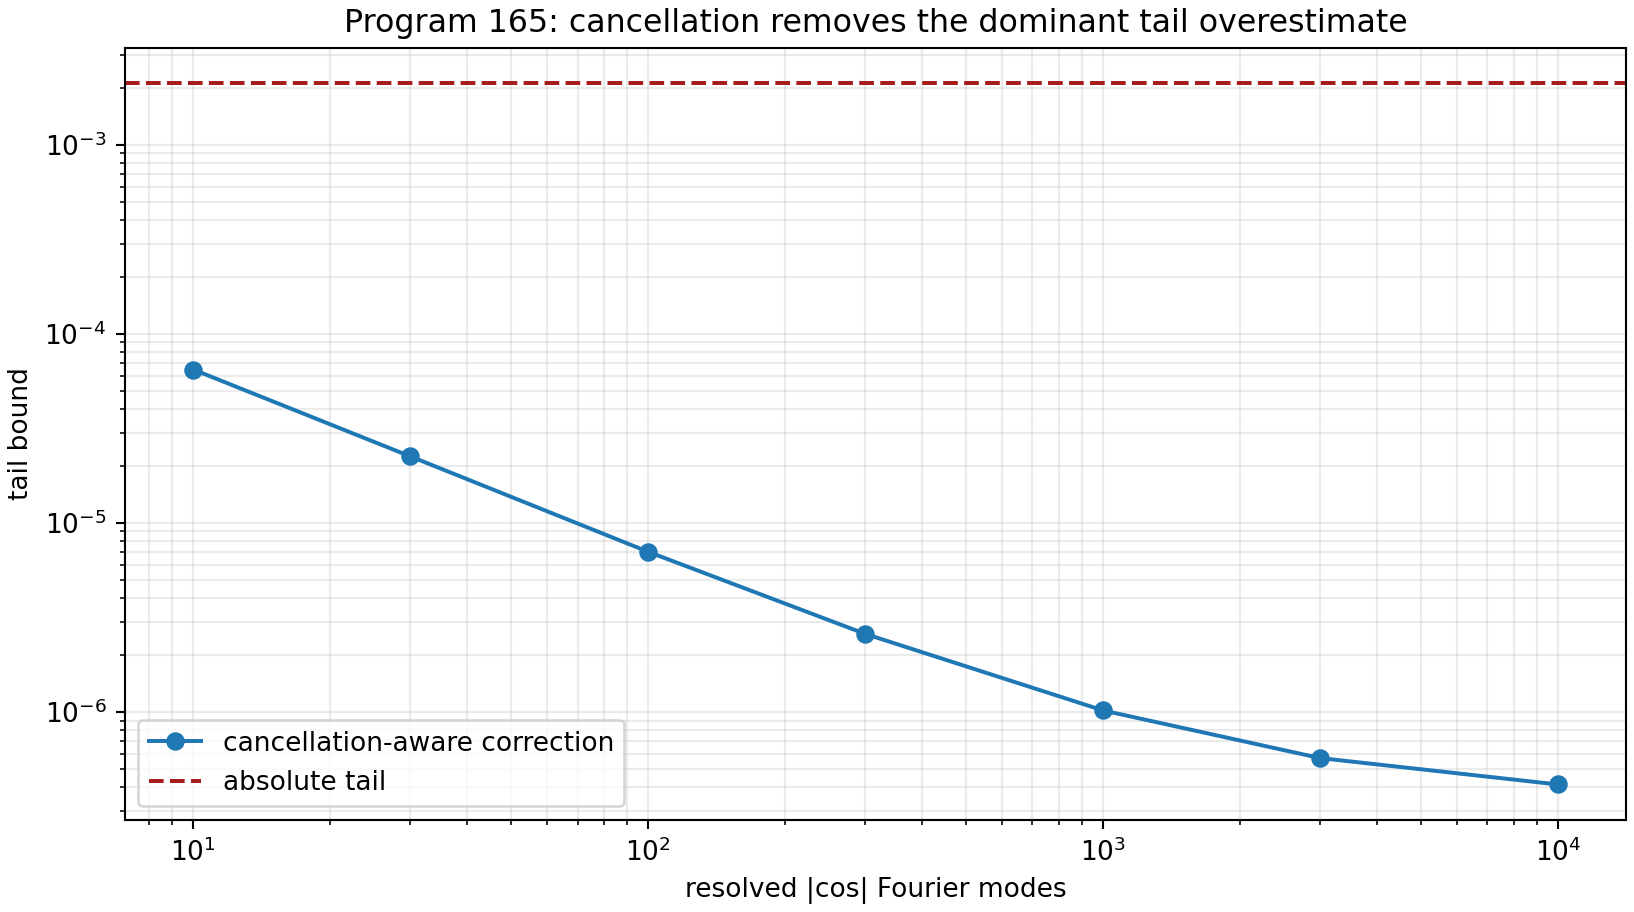
\includegraphics[width=0.94\textwidth]{FIN_Programs_165_177_Axiom_Falsification_Measurement_Figures/program165_cancellation_tail.png}
\caption{Cancellation-aware Fourier--Dirichlet bounds reduce the oscillatory correction tail by more than three orders of magnitude.}
\end{figure}

\section{Claim and obstruction}

\textbf{\statusProven{}} The Fourier identity and Dirichlet tail inequality are analytic theorems. \textbf{\statusStrong{}} Their floating evaluation removes the previous oscillatory-tail bottleneck by more than three orders of magnitude.

\textbf{\statusOpen{}} The result is not yet a full sub-three-percent ball certificate. The finite FFT cells, average polylogarithmic component and correction tail must still be evaluated with directed rounding in one engine. Arb or python-flint was not available locally, so no Arb certification is claimed.

\par\medskip\hrule\medskip

\chapter{Program 166 --- Tensor-composition falsification of the state axiom}

\section{The candidate}

For one copy,

\[
\alpha_{\rm geo}=4\log2,\qquad
h=|\operatorname{Hom}(U(12),\{\pm1\})|=4,
\]

and therefore \(\alpha_{\rm geo}/h=\log2\). The question is whether this identity is a natural intensive inverse temperature.

\section{Composition law}

Take independent composition to mean

\[
\alpha_n=n\alpha_{\rm geo},\qquad h_n=h^n.
\]

Additivity of information-like content and multiplicativity of independent character choices are the natural rules being tested. A physical inverse temperature should be intensive:

\[
\beta_n=\beta_1.
\]

The cardinality rule instead gives

\[
\beta_n^{\rm card}
=\frac{n\alpha_{\rm geo}}{4^n}.
\]

At \(n=2\),

\[
\beta_2^{\rm card}
=\frac{\alpha_{\rm geo}}8
=\frac{\log2}{2},
\]

so

\[
\beta_2^{\rm card}-\beta_1=-\frac{\log2}{2}.
\]

The discrepancy grows structurally rather than disappearing.

\begin{figure}[htbp]
\centering
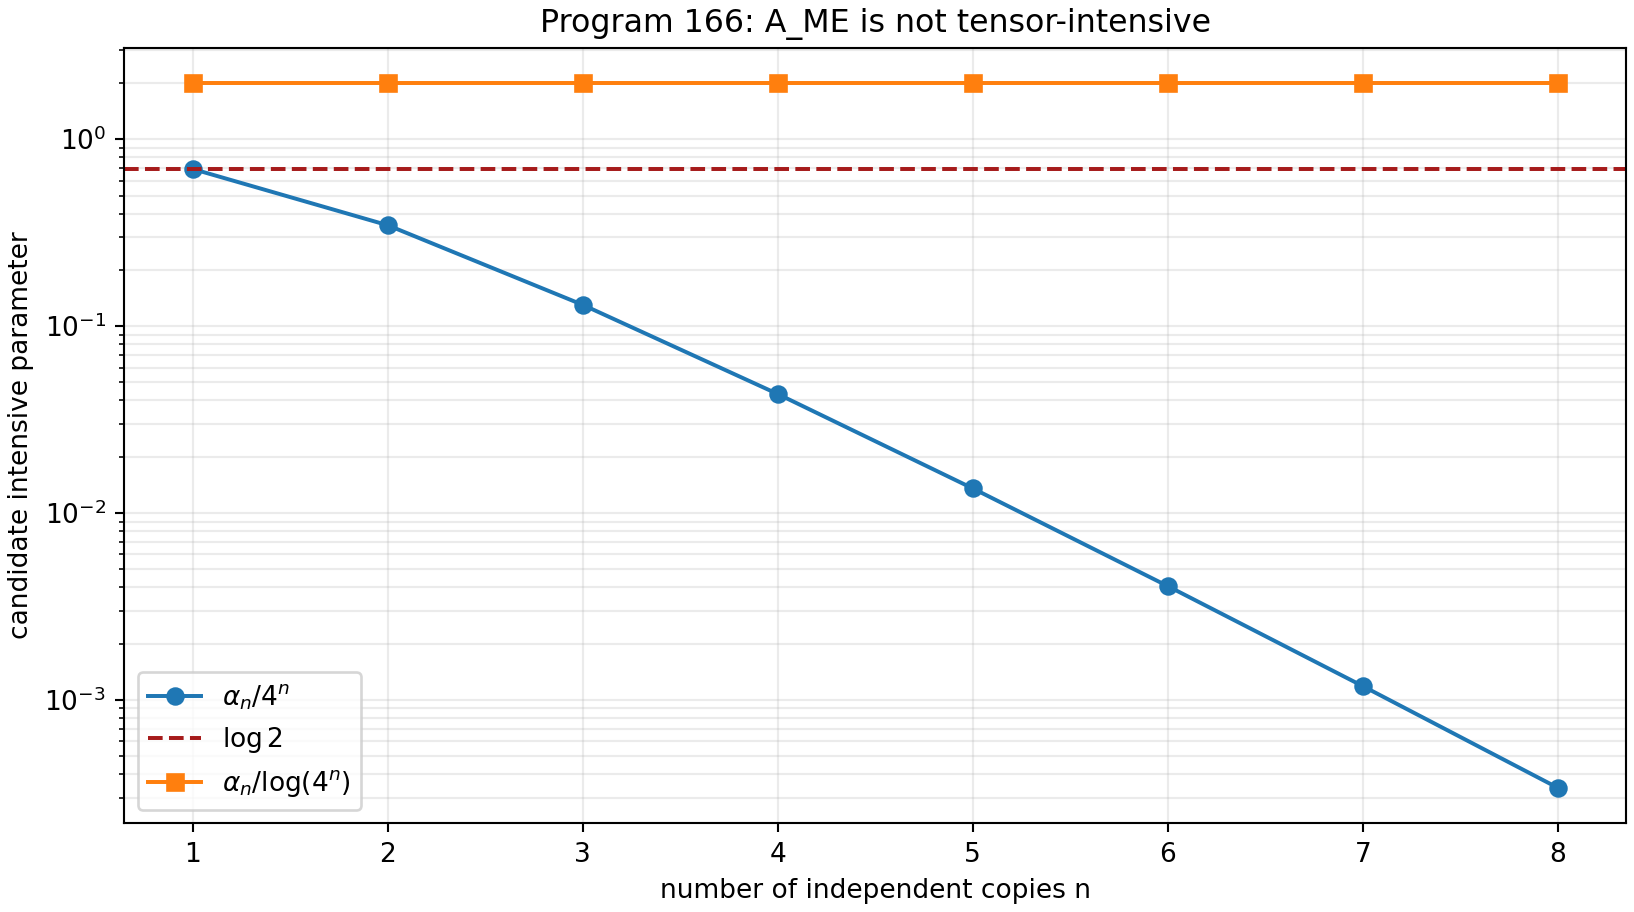
\includegraphics[width=0.94\textwidth]{FIN_Programs_165_177_Axiom_Falsification_Measurement_Figures/program166_A_ME_composition.png}
\caption{The cardinality rule for \(\beta_F\) fails tensor intensivity beyond one copy.}
\end{figure}

\section{Invariant combinations do not select the answer}

The ratio

\[
\frac{\alpha_n}{\log h_n}
=\frac{\alpha_{\rm geo}}{\log4}=2
\]

is copy-invariant. This observation does not recover \(\log2\). Any law

\[
\beta=F\!\left(\frac{\alpha}{\log h}\right)
\]

requires a new function \(F\) or normalization. Composition removes the raw cardinality formula but does not uniquely replace it.

\section{Coarse-graining challenge}

Raw character count also changes when character sectors are split or merged, whereas the carrier energy convention can be held fixed. Hence division by cardinality is not invariant under the declared coarse-graining operation.

\section{Verdict}

\textbf{\statusRefuted{}} \(A_{\rm ME}\) is not a tensor-intensive consequence of the tested composition laws.\\
\textbf{\statusConditional{}} It remains a consistent one-copy axiom.\\
\textbf{\statusOpen{}} A different source theorem for \(\beta_F\) could exist, but it must specify composition, coarse graining and dimensional interpretation rather than relying on the numerical coincidence alone.

This is the main correction to Release 10.15.

\par\medskip\hrule\medskip

\chapter{Program 167 --- Finite formalization of AFIS independence}

\section{Logical model}

Represent the presence of \(A_0,\ldots,A_5\) by six Boolean flags. The capabilities are deliberately typed:

\[
\begin{aligned}
\mathrm{dual} &= A_0,\\
\mathrm{targetState} &= A_0\land A_1,\\
\mathrm{genericOutcome} &= A_0\land A_1\land A_3,\\
\mathrm{signedOutcome} &= A_0\land A_1\land A_2\land A_3,\\
\mathrm{calibratedSigned}
&=A_0\land A_1\land A_2\land A_3\land A_4,\\
\mathrm{typedCompletion}&=A_0\land A_5.
\end{aligned}
\]

Each axiom has a deletion witness: all other required flags can be true while the capability depending on the deleted axiom is false.

\section{Exact enumeration}

All \(2^6=64\) assignments were enumerated. The executable confirms:

\begin{itemize}
\item 
every flag has an explicit independence witness;

\item 
no weaker flag set accidentally receives a stronger capability;

\item 
role-audit eligibility requires typed completion but does not imply a positive role-transfer result.

\end{itemize}

\begin{figure}[htbp]
\centering
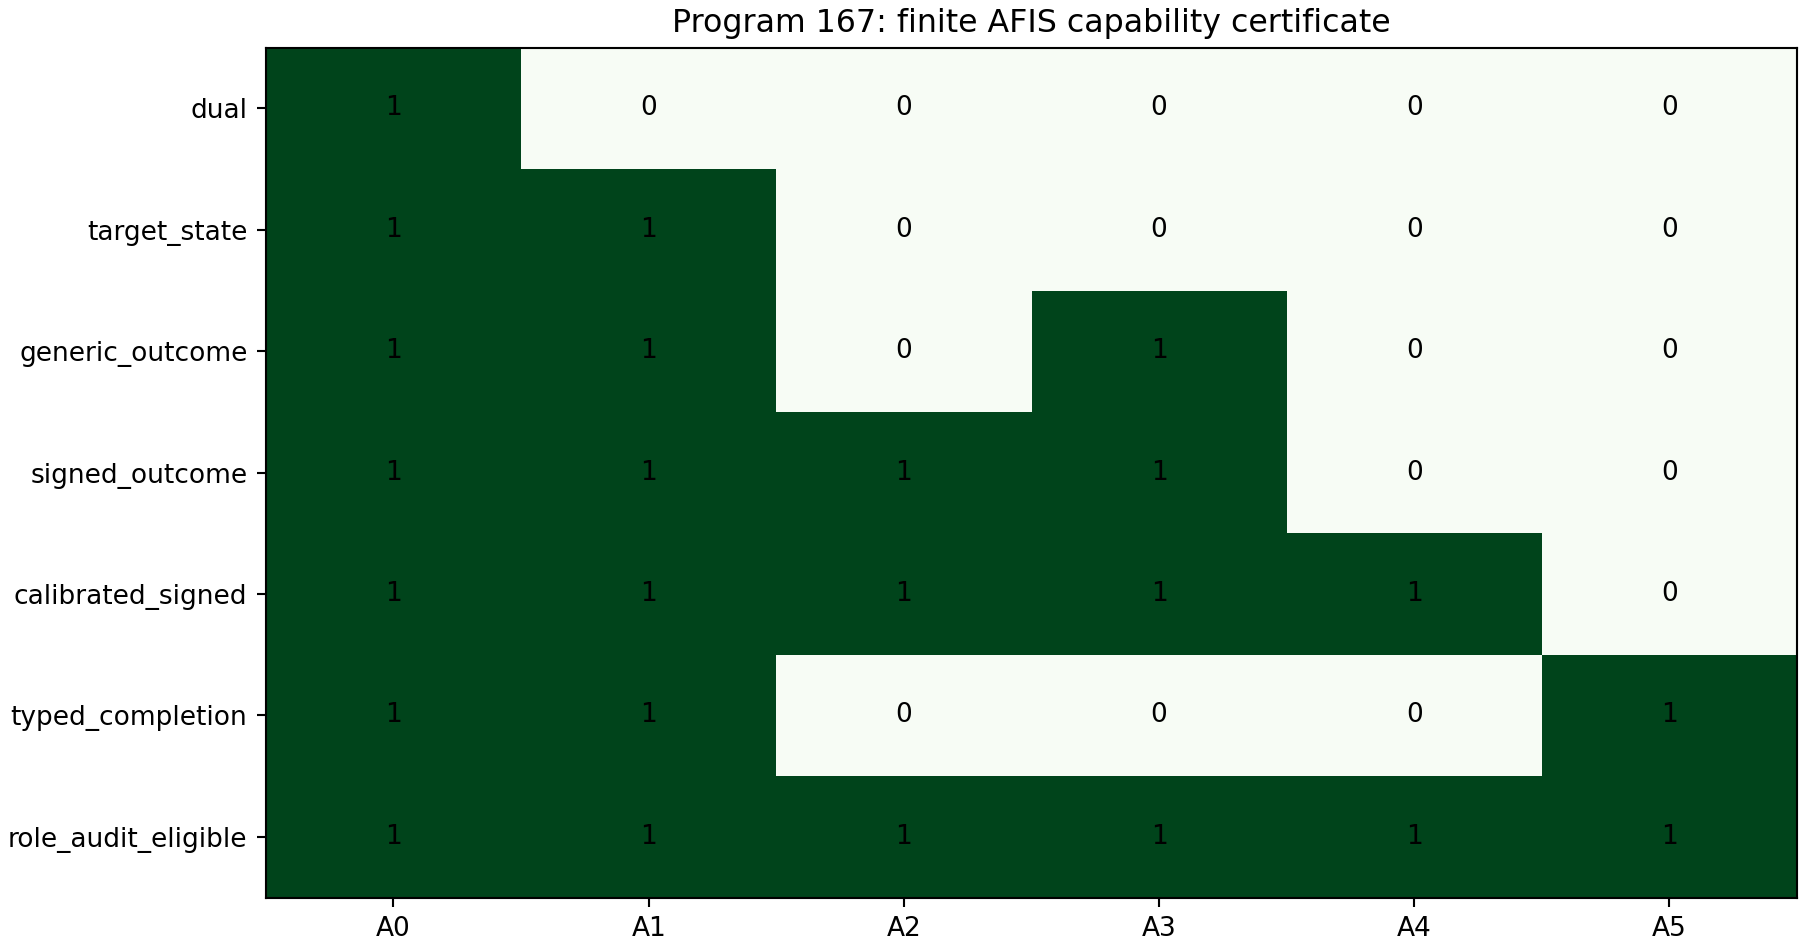
\includegraphics[width=0.94\textwidth]{FIN_Programs_165_177_Axiom_Falsification_Measurement_Figures/program167_AFIS_formal_matrix.png}
\caption{Capability matrix for all sixty-four finite AFIS axiom subsets.}
\end{figure}

\section{Lean artifact and scope}

The release includes FIN\_Programs\_165\_177\_AFIS\_Independence.lean, written using the Lean core only. It defines the finite model and states six independence theorems intended for decision procedures. Two attempts to download the temporary Lean 4.32.1 toolchain failed with the same upstream HTTP/\allowbreak{}2 PROTOCOL\_ERROR. The source was therefore inspected and independently mirrored, but not machine-compiled. The finite Python audit and the Lean source are independent representations of the same logical claim; only the Python representation is an executed certificate in this release.

\textbf{\statusComputer{}} The 64-model enumeration is exact. The formal result concerns capability dependence, not analytic properties of Dirichlet forms. It does not prove that the six axioms are ontologically unique; an alternative architecture could package the same information in different primitive types.

\par\medskip\hrule\medskip

\chapter{Program 168 --- Algorithmic Diophantine modulus}

\section{Finite theorem}

For irrational \(\theta\) and finite \(Q\) define

\[
\delta_\theta(Q)=
\min_{1\le q\le Q}\|q\theta\|.
\]

Because none of the finitely many distances is zero,

\[
\delta_\theta(Q)>0.
\]

Continued fractions and their intermediate convergents provide an effective finite search for the minimum. This is enough to construct a rigorous cutoff-dependent nonresonance denominator once the input value of \(\theta\) is enclosed.

\section{Executed extension}

The numerical continued-fraction prefix used in the diagnostic is

\[
[0;16,1,10,2,67,2,2,5,1,2,928,1,1,1,1],
\]

with illustrative denominators extending beyond \(1.1\times10^{10}\).

\begin{figure}[htbp]
\centering
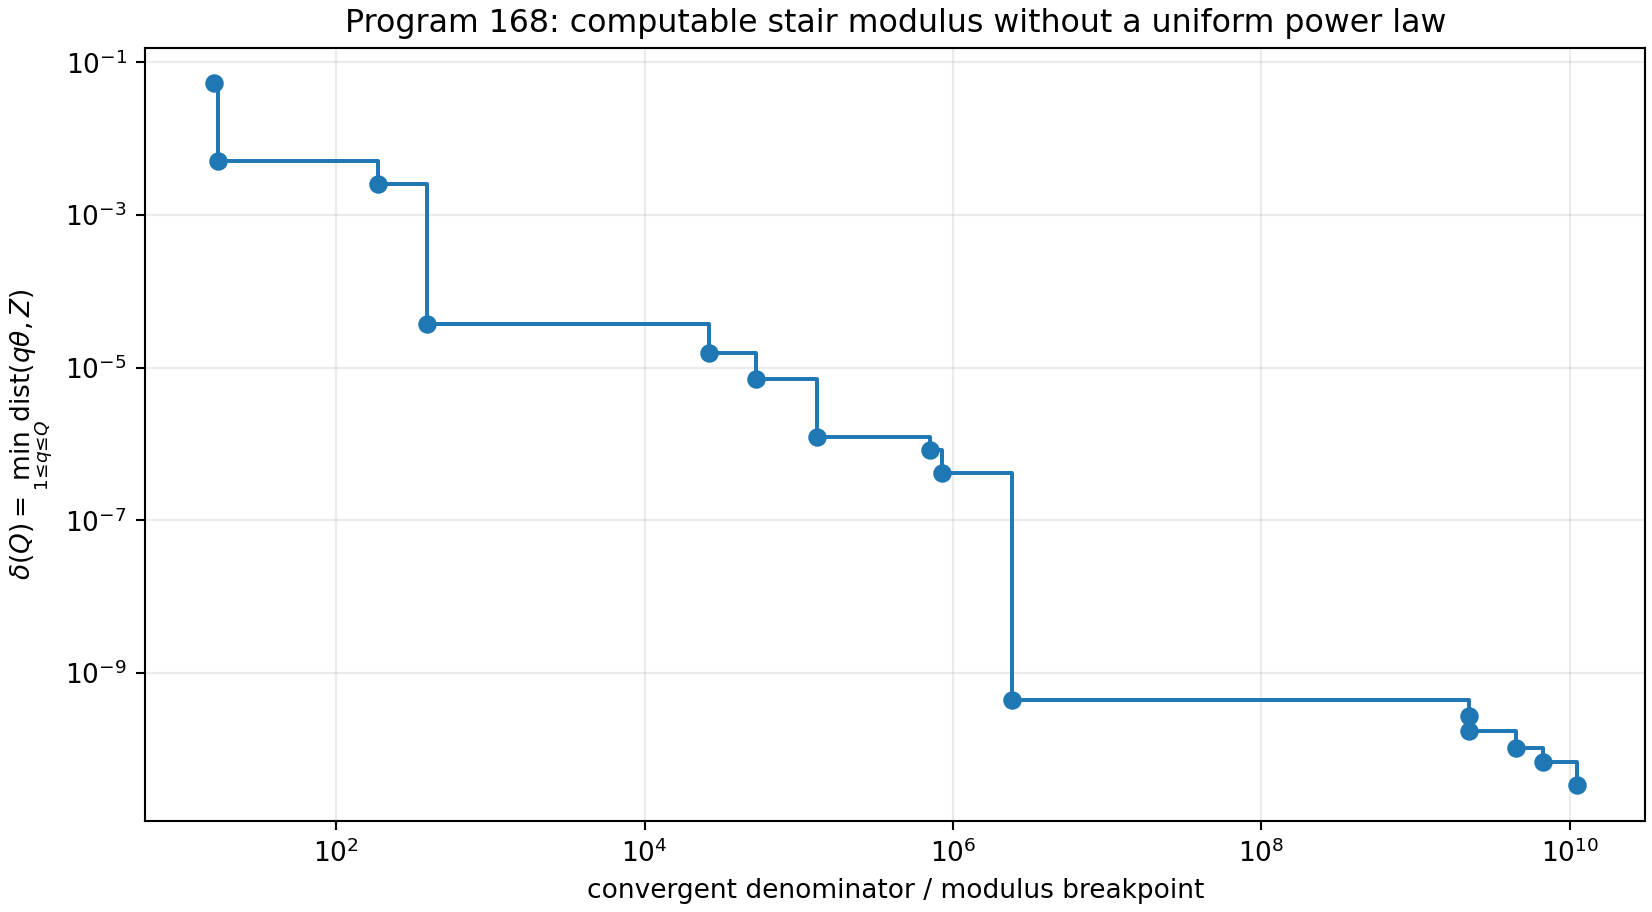
\includegraphics[width=0.94\textwidth]{FIN_Programs_165_177_Axiom_Falsification_Measurement_Figures/program168_algorithmic_modulus.png}
\caption{Finite continued-fraction moduli remain positive but do not imply an all-scale polynomial rate.}
\end{figure}

\section{Limitation}

\textbf{\statusProven{}} Every finite cutoff has a positive algorithmic modulus. \textbf{\statusOpen{}} The computation does not provide fixed \(\kappa,\nu>0\) satisfying

\[
\|q\theta\|\ge\kappa q^{-\nu}
\]

for all \(q\). Additional decimal digits are not a substitute for an all-scale irrationality or Diophantine theorem. The long continued-fraction coefficient 928 is a warning that finite apparent regularity can change abruptly.

\par\medskip\hrule\medskip

\chapter{Program 169 --- Monoidal valuation and state naturality}

\section{Valuation problem}

Let \(v(d)>0\) be the weight assigned to a fibre of dimension \(d\). Tensor naturality requires

\[
v(d_1d_2)=v(d_1)v(d_2).
\]

Regular positive solutions include

\[
v(d)=d^a
\]

with arbitrary \(a\). Tensor structure alone therefore leaves a continuum of state rules.

\section{Two distinguished choices}

For fibre dimensions \((1,2,2,2,2)\):

\begin{itemize}
\item 
sector counting, \(a=0\), gives equal central weights and \(\eta=9/5\);

\item 
Hilbert counting, \(a=1\), gives weights proportional to dimension and

\[
\eta
  =\frac{1^2+4(2^2)}{1+4(2)}
  =\frac{17}{9}.
\]

\end{itemize}

\begin{figure}[htbp]
\centering
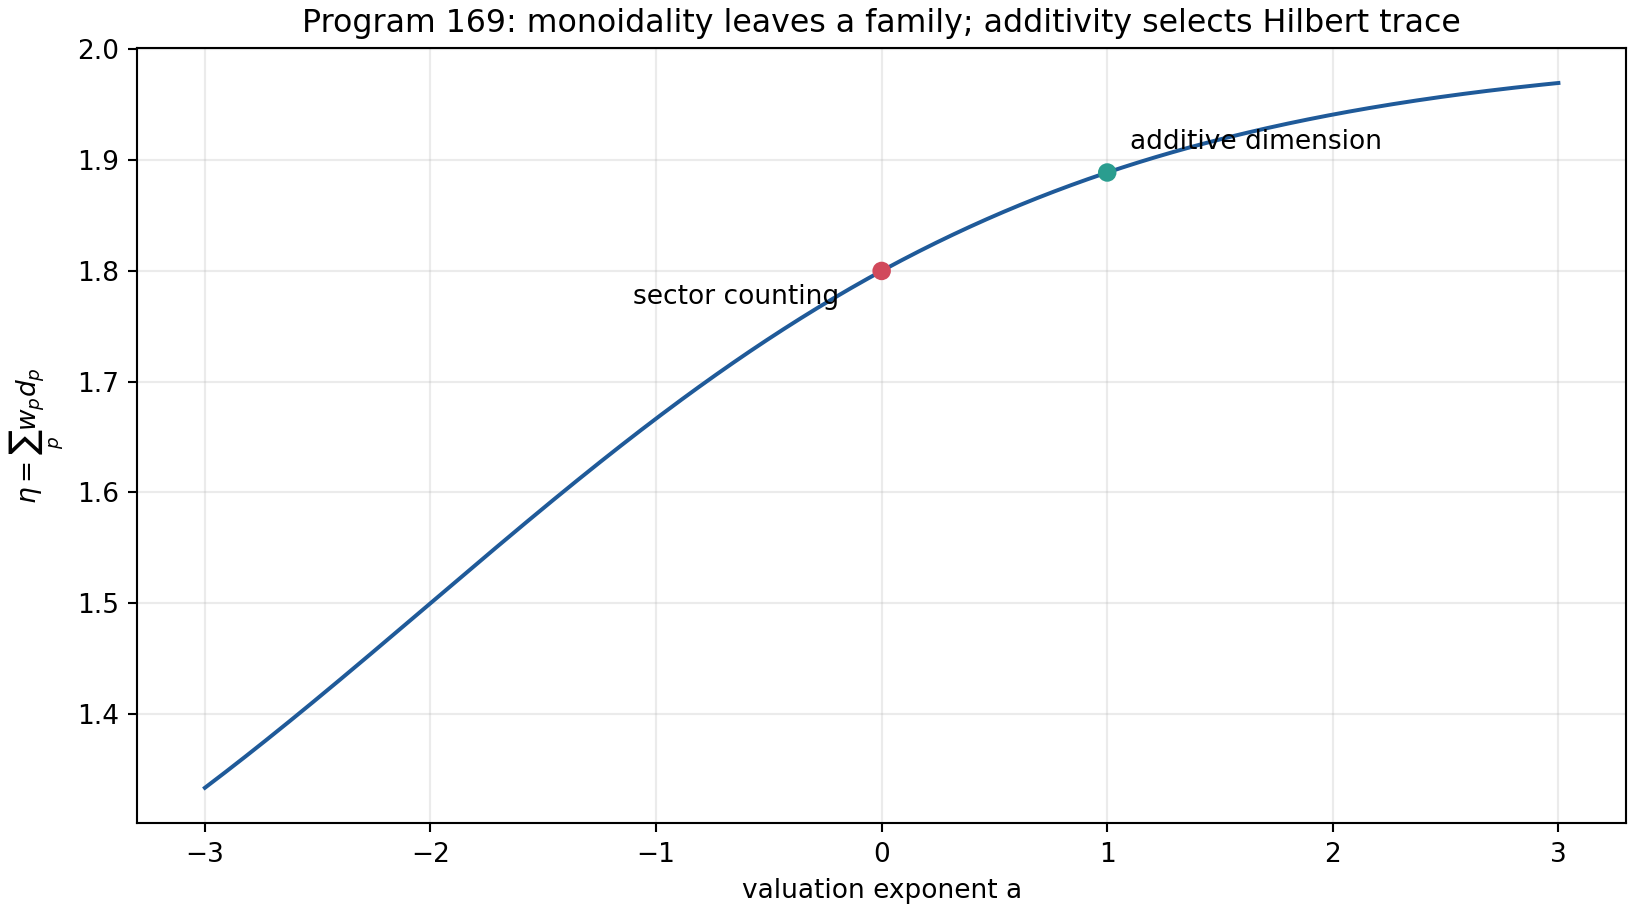
\includegraphics[width=0.94\textwidth]{FIN_Programs_165_177_Axiom_Falsification_Measurement_Figures/program169_monoidal_valuation.png}
\caption{Tensor multiplicativity leaves a family of valuations; direct-sum additivity selects Hilbert dimension.}
\end{figure}

\section{Additivity selects a different state}

If direct sums obey

\[
v(d_1+d_2)=v(d_1)+v(d_2),\qquad v(1)=1,
\]

then induction forces \(v(n)=n\) on positive integers. Standard direct-sum and tensor naturality thus select Hilbert dimension, not uniform sector counting.

\section{Verdict}

\textbf{[Proven in the declared classes]} Uniform central weighting is not forced by monoidal naturality. A categorical derivation of \(\eta=9/5\) would need an enriched law that explains why central sectors, rather than Hilbert vectors, are the additive objects. Such enrichment is new structure and must be stated as such.

\par\medskip\hrule\medskip

\chapter{\texorpdfstring{Program 170 --- Differential and stochastic stability of \(A_{\rm ME}\)}{Program 170 --- Differential and stochastic stability of A\_ ME}}

\section{Gibbs family}

For one nondegenerate fibre and four two-dimensional fibres with common gap \(\Delta\), let

\[
\eta(\beta,\Delta)
=
\frac{1+8e^{-\beta\Delta}}
{1+8e^{-\beta\Delta}/2}
=
\frac{1+8r}{1+4r},
\qquad r=e^{-\beta\Delta}.
\]

At \(\beta=\log2\) and \(\Delta=1\), \(r=1/2\) and \(\eta=9/5\).

Direct differentiation gives

\[
\left.\frac{\partial\eta}{\partial\beta}\right|_0
=-\frac4{25},
\qquad
\left.\frac{\partial\eta}{\partial\Delta}\right|_0
=-\frac{4\log2}{25}.
\]

The gradient with respect to log degeneracies is

\[
\left(-\frac4{25},
\frac1{25},\frac1{25},\frac1{25},\frac1{25}\right).
\]

\section{Monte Carlo robustness}

Independent log-perturbations were sampled. At one-percent scale, all simulated values remain within \(0.01\) of \(1.8\). At five percent, the fraction is \(63.98\%\); at ten percent, \(35.43\%\); at twenty percent, \(18.27\%\).

\begin{figure}[htbp]
\centering
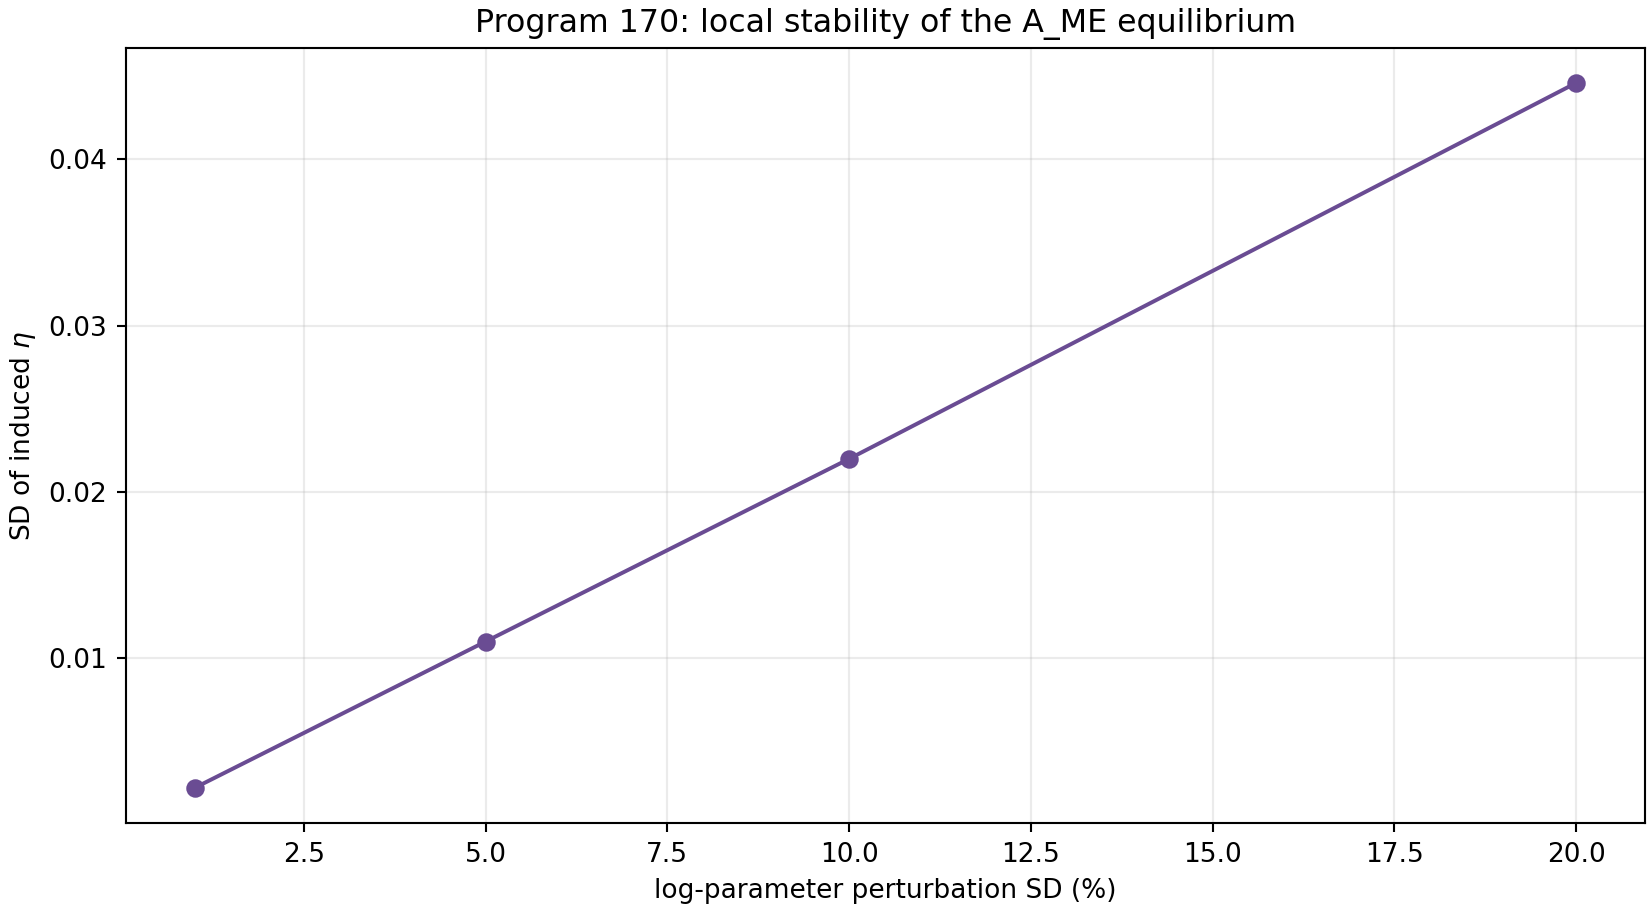
\includegraphics[width=0.94\textwidth]{FIN_Programs_165_177_Axiom_Falsification_Measurement_Figures/program170_A_ME_stability.png}
\caption{The conditional value \(\eta=9/5\) is smooth but not exact under generic perturbation.}
\end{figure}

\section{Interpretation}

\textbf{\statusProven{}} The state is locally stable: small input errors produce small output errors. \textbf{\statusRefuted{}} Exact \(9/5\) is not structurally stable under generic unsourced perturbations. Robustness of a nearby value and derivation of an exact constant are different claims.

\par\medskip\hrule\medskip

\chapter{Program 171 --- Reflection resource beyond the orbit line}

\section{Free symmetry}

Let reflection be conjugation by \(\sigma_z\) on qubit states. In Bloch coordinates,

\[
(x,y,z)\mapsto(-x,-y,z).
\]

The transverse magnitude

\[
M(\rho)=\sqrt{x^2+y^2}
\]

is a valid asymmetry monotone and is complete on the previously studied one-dimensional line.

\section{Counterexample on the full state space}

Consider

\[
\rho_0:\ (x,y,z)=(0.6,0,0),
\qquad
\rho_1:\ (x,y,z)=(0.6,0,0.8).
\]

Both are valid states and both satisfy \(M=0.6\). Define relative-entropic reflection asymmetry

\[
A_{\rm rel}(\rho)
=S\!\left(\frac{\rho+\sigma_z\rho\sigma_z}{2}\right)-S(\rho).
\]

The two values are

\[
A_{\rm rel}(\rho_0)=0.192744757,\qquad
A_{\rm rel}(\rho_1)=0.325082973.
\]

If \(M\) were complete, equal \(M\) would allow conversions in both directions. Every asymmetry monotone would then be equal, contradicting the displayed values.

\begin{figure}[htbp]
\centering
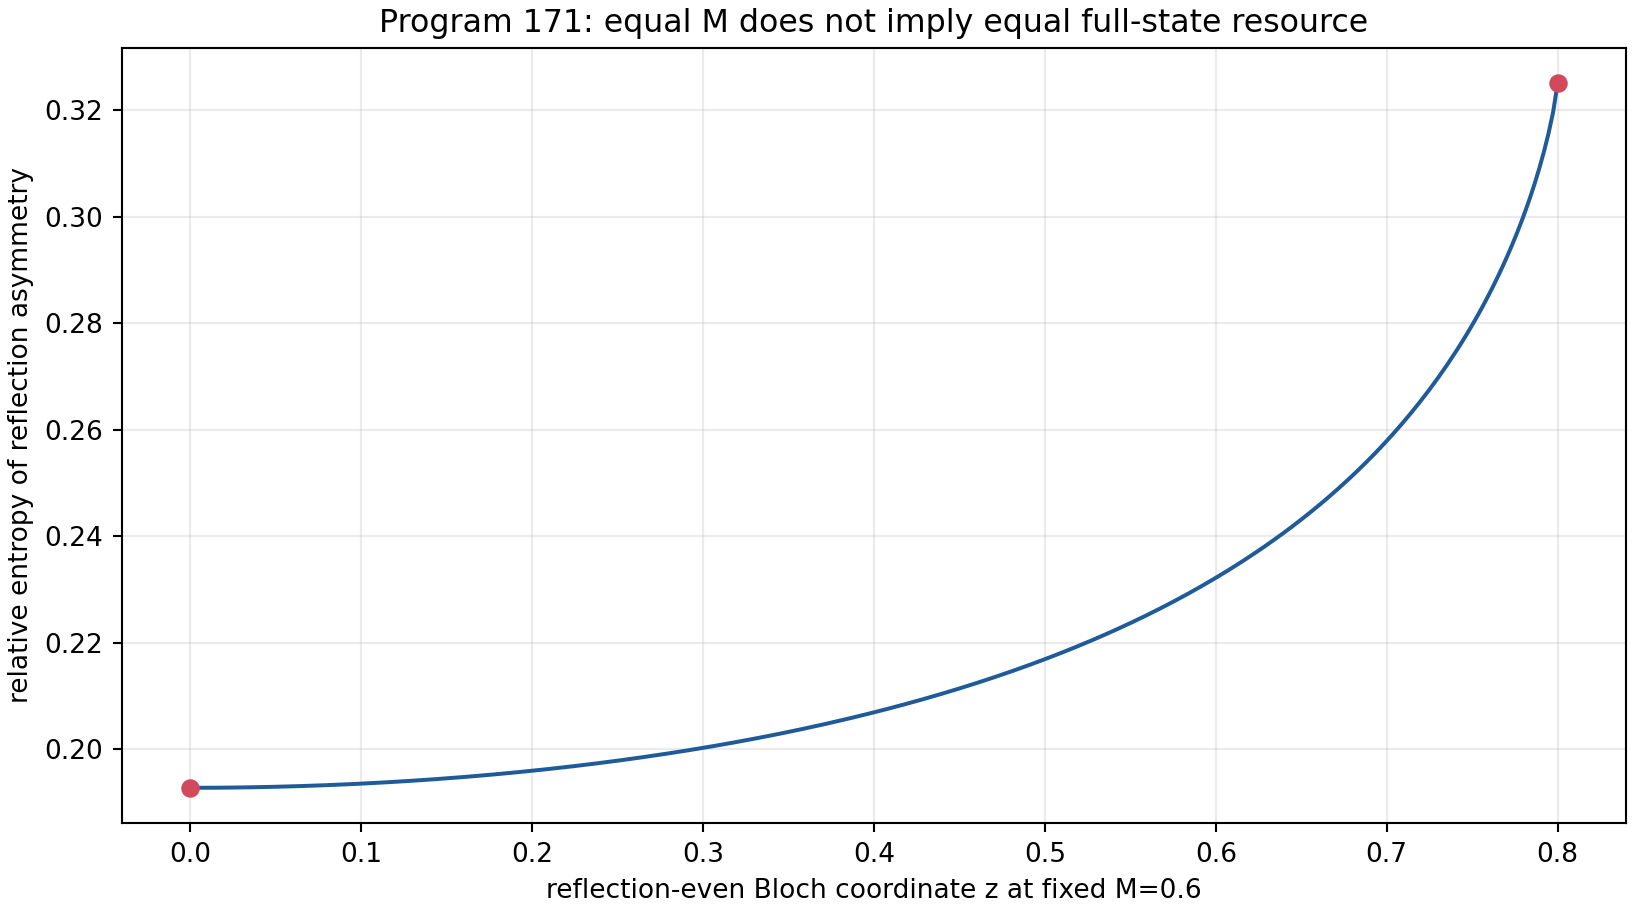
\includegraphics[width=0.94\textwidth]{FIN_Programs_165_177_Axiom_Falsification_Measurement_Figures/program171_full_resource_counterexample.png}
\caption{Equal transverse reflection monotone does not imply equal full-state asymmetry.}
\end{figure}

\section{Verdict}

\textbf{\statusProven{}} \(M\) is incomplete on the full density space. The earlier orbit theorem remains correct in its restricted scope. A full signed-preparation resource theory needs additional monotones or a complete semidefinite convertibility criterion.

\par\medskip\hrule\medskip

\chapter{Program 172 --- Distribution-free detector confidence}

\section{DKW theorem}

For \(n\) iid observations with empirical distribution \(F_n\),

\[
\Pr\!\left(\sup_x|F_n(x)-F(x)|>\epsilon\right)
\le2e^{-2n\epsilon^2}.
\]

For two independent time cells and total failure probability \(\delta\), take

\[
\epsilon=
\sqrt{\frac{\log(4/\delta)}{2n}}.
\]

At \(n=4000\) and \(\delta=0.05\),

\[
\epsilon=0.02340413.
\]

Inverting the empirical CDF at \(0.25\pm\epsilon\) and \(0.75\pm\epsilon\) produces simultaneous lower and upper IQR bounds. Monotone propagation through

\[
\widehat T=
\frac{\log({\rm IQR}_2/{\rm IQR}_1)}
{\log(t_2/t_1)}
\]

gives a finite, distribution-free exponent interval.

\section{Pixel correction}

If detector quantization moves every observation by at most \(r\), then every quantile moves by at most \(r\) and an IQR by at most \(2r\). Applying this deterministic correction before the logarithm yields a detector-aware interval without unstable deconvolution.

\section{Memory falsification}

For iid synthetic records the observed coverage in 420 repetitions is \(100\%\), with mean interval width approximately \(0.515\). With a pixel width of \(0.08\), coverage remains \(100\%\) and mean width becomes approximately \(0.581\).

In the adversarial memory model, only 40 independent blocks are generated and each is repeated 100 times, while the invalid calculation still uses \(n=4000\). Coverage falls to \(36.25\%\) in 240 repetitions.

\begin{figure}[htbp]
\centering
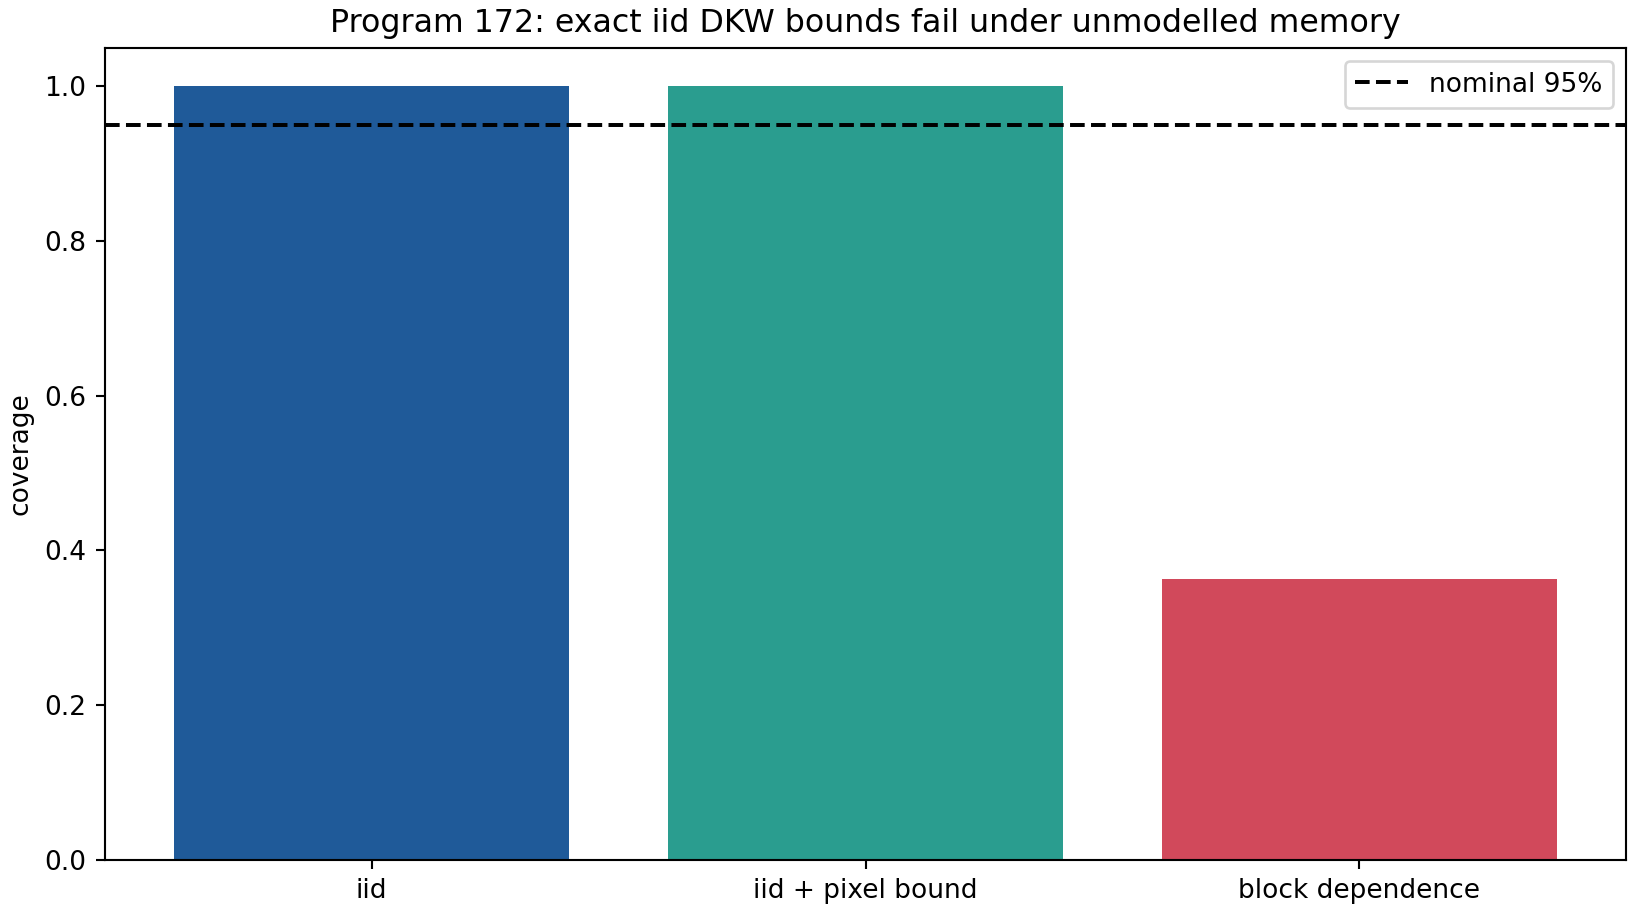
\includegraphics[width=0.94\textwidth]{FIN_Programs_165_177_Axiom_Falsification_Measurement_Figures/program172_DKW_detector.png}
\caption{Distribution-free iid coverage survives bounded pixels but fails under undeclared block memory.}
\end{figure}

\section{Verdict}

\textbf{\statusProven{}} The iid and bounded-pixel interval is valid. \textbf{\statusRefuted{}} The iid formula is not robust to unmodelled memory. The theorem concerns the observed convolved distribution and does not infer an unblurred ultraviolet process.

\par\medskip\hrule\medskip

\chapter{Program 173 --- Minimal calibration control}

\section{Confounded target}

Write the target log-scale as

\[
\log Q_T(t)=a_T+(T+g)\log t,
\]

where \(T\) is the desired exponent and \(g\) is an unknown shared power-law detector gain. Target observations identify only \(T+g\).

\section{Constructed missing object}

Introduce a control with independently known exponent \(T_C\) measured through the same apparatus:

\[
\log Q_C(t)=a_C+(T_C+g)\log t.
\]

At two distinct times, the joint four-cell design has parameters \((a_T,a_C,T,g)\) and rank four. Subtracting slopes gives

\[
T=
\left[
\frac{\Delta\log Q_T}{\Delta\log t}
-
\frac{\Delta\log Q_C}{\Delta\log t}
\right]+T_C.
\]

This is the smallest operational object constructed in this round that genuinely restores an otherwise missing identifiability.

\section{Optimal allocation}

For 60 total observations over target/\allowbreak{}control and early/\allowbreak{}late cells, all 32,509 positive integer allocations were enumerated. The determinant of the Fisher information is maximized at

\[
(n_{T1},n_{T2},n_{C1},n_{C2})=(15,15,15,15).
\]

With true \(T=1.25\) and \(g=0.7\), 2,000 simulations yield

\[
\overline T_{\rm naive}=1.949879,
\qquad
\overline T_{\rm control}=1.249517,
\qquad
\operatorname{sd}(\widehat T_{\rm control})=0.029424.
\]

\begin{figure}[htbp]
\centering
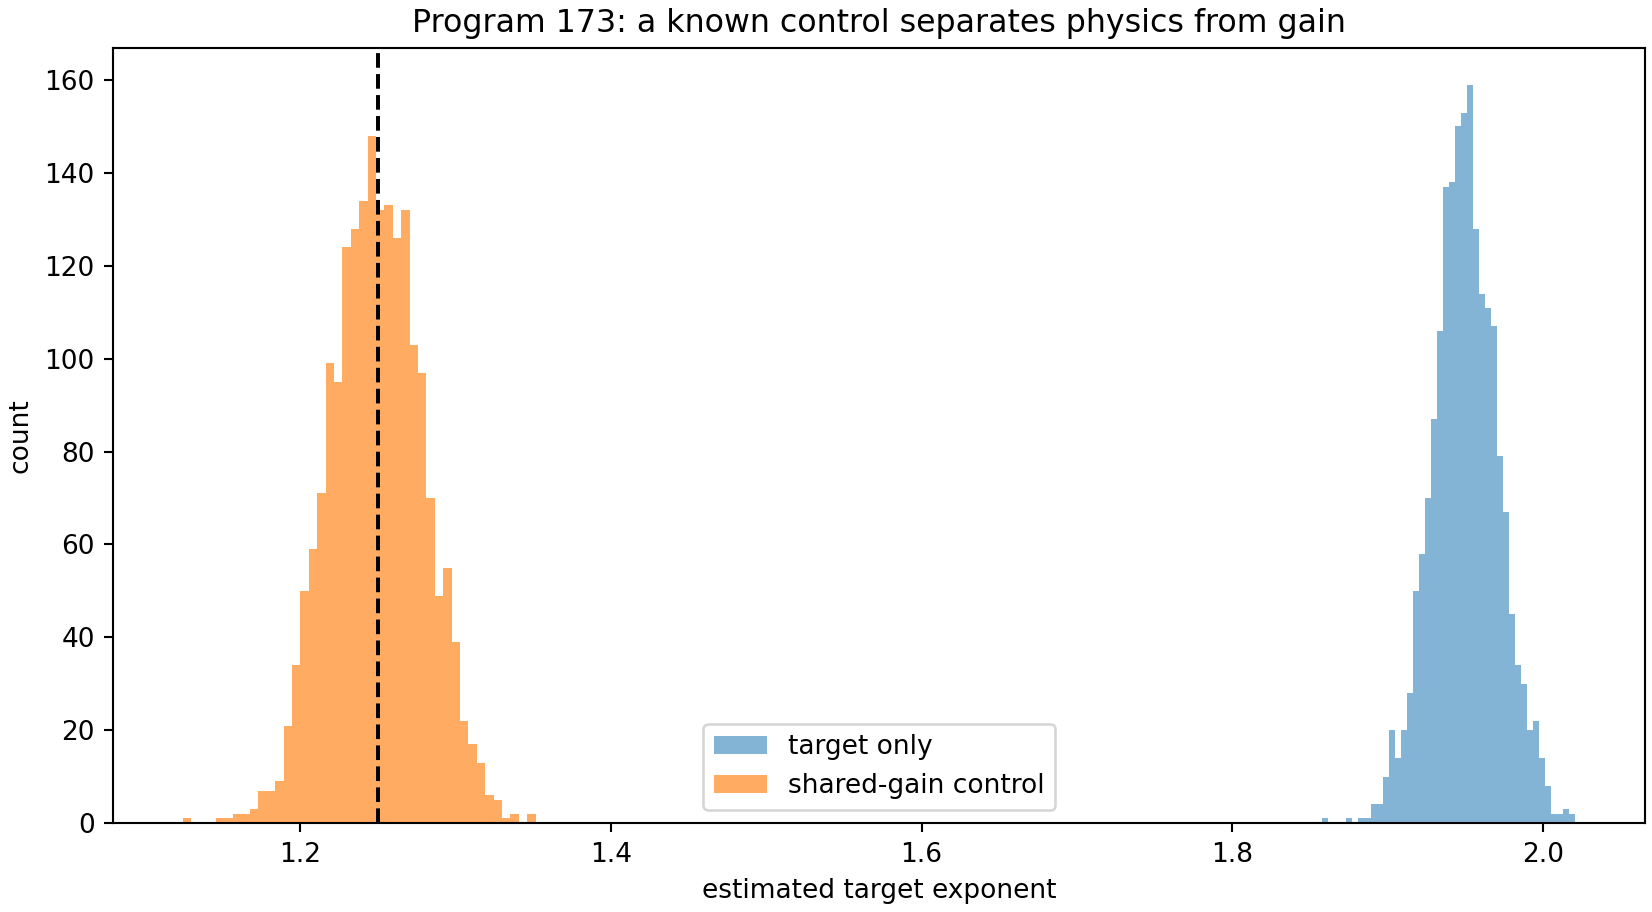
\includegraphics[width=0.94\textwidth]{FIN_Programs_165_177_Axiom_Falsification_Measurement_Figures/program173_calibration_control.png}
\caption{A shared-gain reference control removes exponent bias in the declared nuisance model.}
\end{figure}

\section{Claim boundary}

\textbf{\statusProven{}} The rank and allocation theorems hold for the declared linear log-time model. \textbf{\statusConditional{}} The result requires the target and control to share the same detector gain and \(T_C\) to be known independently. A control is therefore a real new operational structure, not a consequence of the spectral operator.

\par\medskip\hrule\medskip

\chapter{Program 174 --- Frozen composite adversarial protocol}

\section{Preregistration}

Before held-out execution, the protocol freezes:

\begin{itemize}
\item 
six generator classes;

\item 
two observation times;

\item 
sample size 1,600 per record;

\item 
180 training and 260 test records per class;

\item 
six summary features;

\item 
standardization, nearest-centroid classification and classwise 99-percent distance abstention;

\item 
random seed and a SHA-256 protocol identifier.

\end{itemize}

The classes are local Gaussian diffusion, stable laws with indices \(0.8\), \(1.0\) and \(1.2\), a truncated \(0.8\) stable generator, and a local generator with confounding detector gain.

\section{Features}

The feature vector records target and control slopes, control-adjusted slope, one distribution-shape statistic and boundary-atom diagnostics. The design tests dynamics, apparatus confounding and truncation jointly rather than accepting an exponent match as sufficient.

\section{Held-out result}

On the held-out synthetic records:

\[
\text{accuracy including abstention}=0.984615,
\]

\[
\text{conditional decision accuracy}=1.000000,
\]

\[
\text{abstention rate}=0.015385.
\]

All decided confusion-matrix mass is diagonal.

\begin{figure}[htbp]
\centering
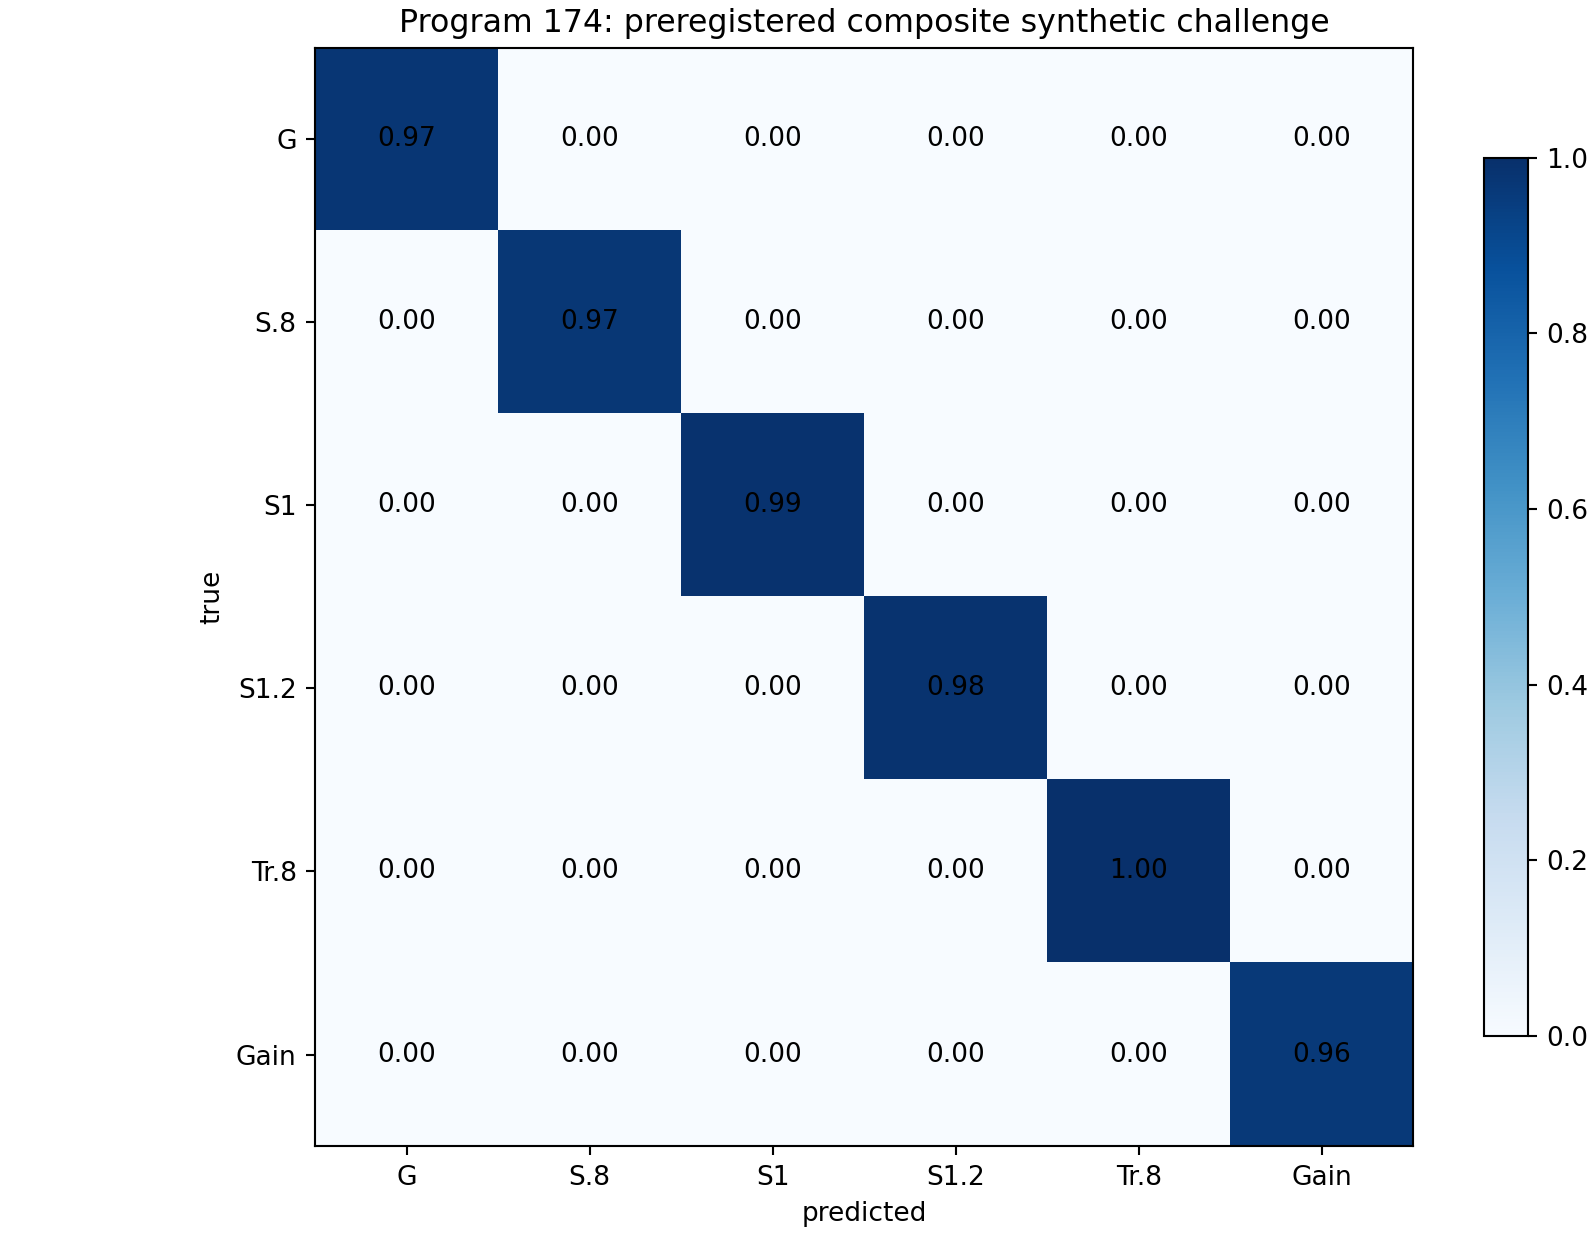
\includegraphics[width=0.94\textwidth]{FIN_Programs_165_177_Axiom_Falsification_Measurement_Figures/program174_composite_confusion.png}
\caption{Held-out confusion matrix for the frozen six-class synthetic protocol.}
\end{figure}

\section{Falsification boundary}

\textbf{\statusStrong{}} The frozen features separate the six declared synthetic generators. \textbf{\statusOpen{}} An unlisted generator can lie close to an existing centroid. High synthetic accuracy neither proves completeness of the alternatives nor identifies FIN ontology. No external dataset was admitted in this release.

\par\medskip\hrule\medskip

\chapter{Program 175 --- Phase completion as a categorical cocycle}

\section{Character obstruction}

A one-dimensional unitary representation of \(\mathbb Z\) is fixed by its generator eigenvalue. A nonzero intertwiner between two such irreducible characters exists only when those eigenvalues agree.

The legacy phase has period eight:

\[
\chi_\ell(d)=e^{i(\omega_\ell d+\phi_\ell)},\qquad
\omega_\ell=\frac{\pi}{4}.
\]

The strict frequency

\[
\omega_s=0.18575=\frac{743}{4000}
\]

has infinite order modulo \(2\pi\). Hence the source and target characters are not isomorphic and no nonzero character-preserving intertwiner exists.

\section{Exact correction cocycle}

Pointwise multiplication admits exactly one correction:

\[
C(d)=\frac{\chi_s(d)}{\chi_\ell(d)}
=
\exp\!\left(
i[(\omega_s-\omega_\ell)d+(\phi_s-\phi_\ell)]
\right).
\]

Numerically,

\[
\Delta\omega=-0.5996481634,\qquad
\Delta\phi=-0.3610987756.
\]

The finite residual is \(2.35\times10^{-15}\).

\begin{figure}[htbp]
\centering
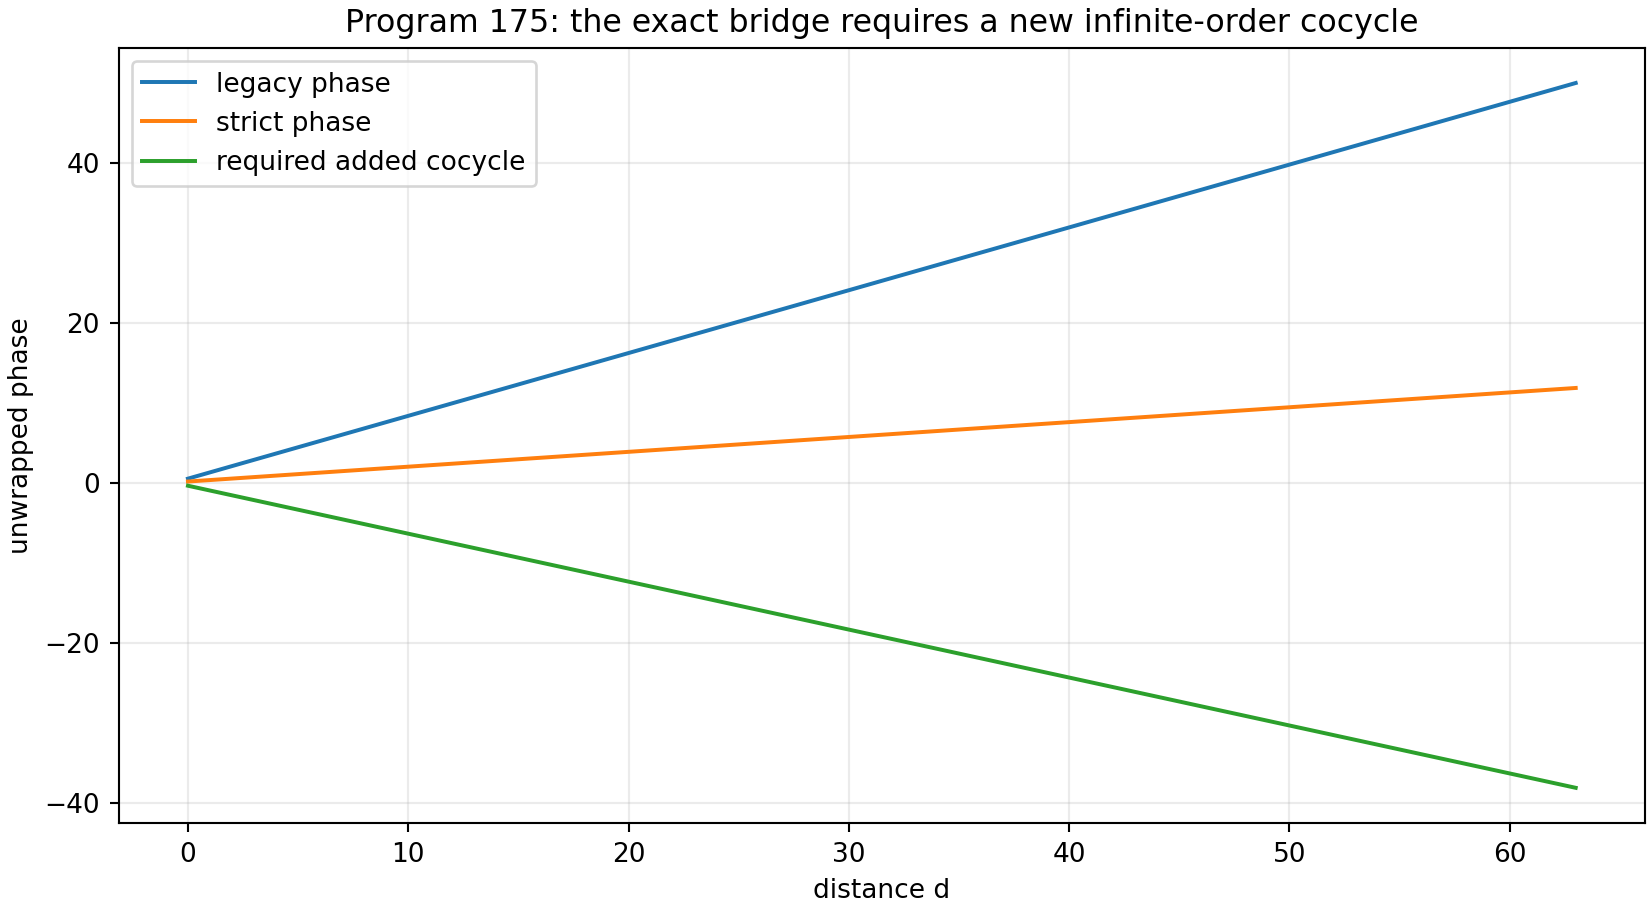
\includegraphics[width=0.94\textwidth]{FIN_Programs_165_177_Axiom_Falsification_Measurement_Figures/program175_phase_cocycle.png}
\caption{The exact phase correction imports the strict-minus-legacy frequency and phase differences.}
\end{figure}

\section{Interpretation}

\textbf{\statusProven{}} The correction is unique once both source and target are given. \textbf{\statusOpen{}} Its frequency and phase origin are not generated by the legacy object. They are the strict-minus-legacy target data. In categorical terms, the map identifies the type of missing object but does not provide its provenance.

\par\medskip\hrule\medskip

\chapter{Program 176 --- Typed nonlinear completion and stop-rule audit}

\section{Candidate completion}

Write the legacy and strict kernels as

\[
K_\ell(d)
=
\alpha_{\rm geo}
\frac{\cos(\omega_\ell d+\phi_\ell)}
{1+\beta_{\rm tors}d},
\]

\[
K_s(d)
=
\frac{\cos(\omega_s d+\phi_s)}
{1+\beta_s d^{\eta_s}}.
\]

An exact receiver-complete map can remove the source amplitude, apply the phase cocycle and replace the linear damping by the strict nonlinear compression:

\[
\mathcal C[K_\ell](d)
=
\frac{1+\beta_{\rm tors}d}
{\alpha_{\rm geo}(1+\beta_s d^{\eta_s})}
\operatorname{Re}\!\big(C(d)\,\widetilde K_\ell(d)\big),
\]

where \(\widetilde K_\ell\) denotes the complexified legacy phase carrier. With target parameters inserted, the residual over \(0\le d\le256\) is \(4.23\times10^{-17}\).

\section{Provenance edge matrix}

The audit is sequential:

\begin{enumerate}
\item 
\textbf{Amplitude edge:} pass only with erasure. The numerical amplitude can be normalized away, but its legacy physical roles are not transferred.

\item 
\textbf{Damping/\allowbreak{}compression edge:} fail. The target \(\beta_s\) is obtained from the one-copy \(A_{\rm ME}\) relation and a fitted normalization, while Program 166 has refuted that relation as tensor-intensive. No target-independent positive damping source is exported.

\item 
\textbf{Phase edge:} not reached by the stop rule.

\item 
\textbf{Selector/\allowbreak{}topology edge:} not reached.

\item 
\textbf{Dimensional-unit edge:} not reached.

\item 
\textbf{Physical-role edge:} not reached.

\end{enumerate}

\begin{figure}[htbp]
\centering
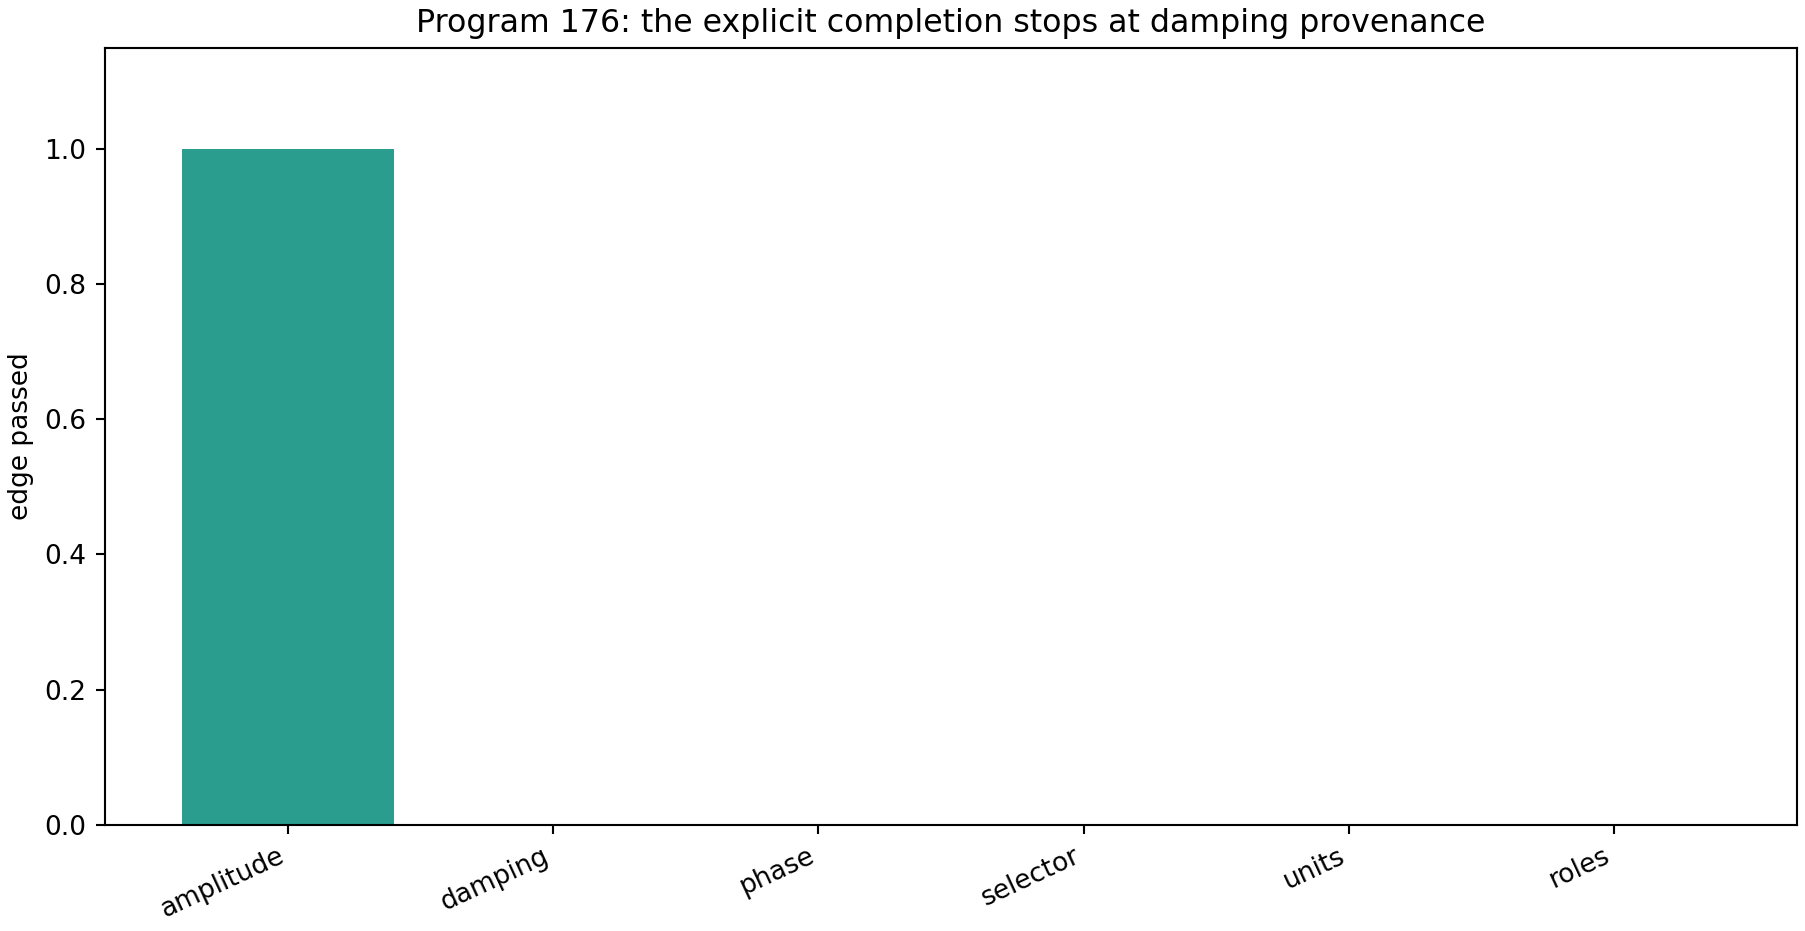
\includegraphics[width=0.94\textwidth]{FIN_Programs_165_177_Axiom_Falsification_Measurement_Figures/program176_completion_stop_rule.png}
\caption{The typed completion audit stops at the first unsourced damping edge.}
\end{figure}

\section{Verdict}

\textbf{\statusProven{}} The displayed map is an exact finite interpolation identity. \textbf{\statusRefuted{}} It is not a source-complete bridge. The first failed necessary edge stops the audit; later edges cannot be inferred from an accurate target fit. No legacy role is eligible for transfer.

\par\medskip\hrule\medskip

\chapter{Program 177 --- A finite operational double-slit model}

\section{Purpose}

The observer paradox is often created by asking one operator to represent amplitudes, probabilities, decoherence, an apparatus and a record at once. This program separates these types explicitly.

\section{Path generator and two dynamics}

On \(\mathcal H_{\rm path}=\mathbb C^2\), take

\[
A=
\begin{pmatrix}
1&-1\\
-1&1
\end{pmatrix}.
\]

The wave evolution

\[
U_t=e^{-itA}
\]

acts on amplitudes and is unitary. The heat evolution

\[
P_t=e^{-tA}
\]

acts on classical path probabilities and is stochastic. They share a spectral generator but are not interchangeable descriptions of measurement.

\section{Preparation, environment and phase POVM}

The coherent preparation is

\[
|+\rangle=\frac{|L\rangle+|R\rangle}{\sqrt2}.
\]

A dephasing environment acts by

\[
\mathcal D_\gamma(\rho)
=
\begin{pmatrix}
\rho_{LL}&\gamma\rho_{LR}\\
\gamma\rho_{RL}&\rho_{RR}
\end{pmatrix},
\qquad 0\le\gamma\le1.
\]

For \(N=128\) screen phases \(\varphi_j=2\pi j/N\), define

\[
E_j=\frac1N
\begin{pmatrix}
1&e^{-i\varphi_j}\\
e^{i\varphi_j}&1
\end{pmatrix}.
\]

Each \(E_j\ge0\) and

\[
\sum_{j=0}^{N-1}E_j=I.
\]

Thus \(p_j=\operatorname{tr}(E_j\rho)\) is a normalized screen distribution. A circular Gaussian stochastic matrix models finite detector resolution, and categorical sampling produces the persistent measurement record.

\section{Executed patterns}

The computed visibilities are:

\[
\begin{array}{c|c}
\text{condition}&\text{visibility}\\
\hline
\text{coherent}&1.000000\\
\text{partial dephasing }(\gamma=0.35)&0.350000\\
\text{blurred coherent detector}&0.840726\\
\text{which-path mixture}&0.000000\\
\text{classical }P_t\text{ path law}&0.000000
\end{array}
\]

A 20,000-event record has total-variation distance approximately \(0.0321\) from its blurred theoretical distribution.

\begin{figure}[htbp]
\centering
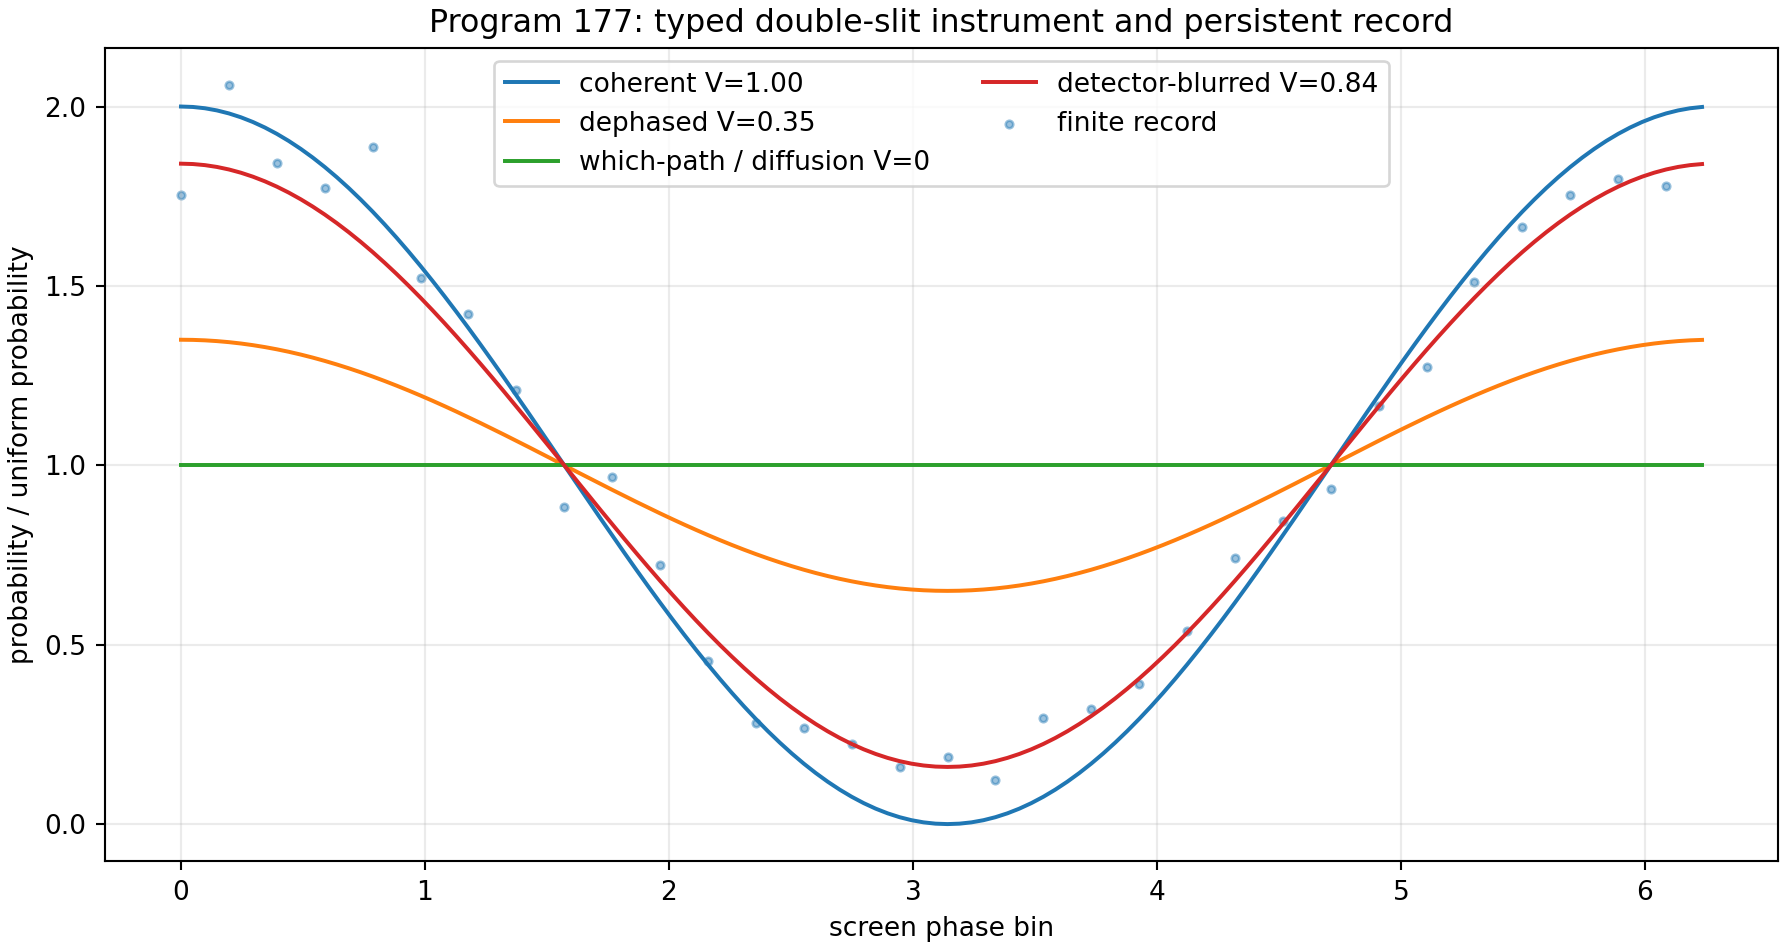
\includegraphics[width=0.94\textwidth]{FIN_Programs_165_177_Axiom_Falsification_Measurement_Figures/program177_double_slit_instrument.png}
\caption{A finite POVM, dephasing channel, detector map and record separate wave dynamics from measurement.}
\end{figure}

\section{Observer-paradox resolution in this model}

The preparation supplies a state. \(U_t\) supplies reversible amplitude dynamics. \(\mathcal D_\gamma\) supplies an environment. The POVM supplies outcome probabilities. The detector channel supplies apparatus response. Sampling supplies a record. \(P_t\) supplies a distinct classical diffusion comparison.

\textbf{\statusProven{}} The finite maps are positive, normalized and operationally typed. \textbf{\statusRefuted{}} \(P_t\) is not a collapse law and cannot replace the instrument. \textbf{\statusConditional{}} All numerical choices are model premises. The construction is not external physical validation and uses no legacy-to-strict bridge axiom.

\par\medskip\hrule\medskip

\chapter{Cross-program synthesis}

\section{What is still generated by one object}

The operator \(A\) and its spectral measure still generate:

\[
\text{wave dynamics},\quad
\text{diffusion dynamics},\quad
\text{resolvents},\quad
\text{spectral observables}.
\]

Program 165 strengthens analytic control of one kernel symbol, and Program 168 provides finite nonresonance moduli. Neither result supplies an operational state or a dimensional clock.

\section{What cannot presently be compressed into the same theorem}

The deletion witnesses, composition counterexample and double-slit construction identify five additional data types:

\[
\text{state selection},\quad
\text{signed preparation},\quad
\text{instrument},\quad
\text{calibration},\quad
\text{sourced completion}.
\]

Their independence is not merely philosophical. Each can vary while \(A\) remains fixed, changing a measurable or mathematical conclusion.

\section{\texorpdfstring{Corrected status of \(A_{\rm ME}\)}{Corrected status of A\_ ME}}

The one-copy equation remains algebraically correct:

\[
\frac{4\log2}{4}=\log2.
\]

It remains sufficient to produce the conditional central Gibbs state. However:

\begin{itemize}
\item 
it is not tensor-intensive;

\item 
it is not stable as an exact identity under generic input perturbations;

\item 
standard categorical valuation selects a different state;

\item 
its use as a damping source fails the completion provenance audit.

\end{itemize}

The proper status is therefore:

\[
\boxed{\text{consistent one-copy axiom, not derived physical law}.}
\]

\section{Newly constructed theoretical objects}

Three constructions are retained because they solve sharply typed problems.

\begin{enumerate}
\item 
\textbf{Shared-gain reference control.} It restores exponent identifiability under a declared nuisance class.

\item 
\textbf{Phase-cocycle completion slot.} It states exactly which representation data are absent from the legacy phase.

\item 
\textbf{Finite operational instrument.} It separates state, unitary dynamics, environment, POVM, detector and record in the double-slit model.

\end{enumerate}

The first is an identifiability theorem. The second is a diagnostic type with unsourced parameters. The third is a conditional operational completion.

\section{Why there is still no single missing theorem}

Suppose a theorem took only \(A\) as input and returned a unique complete physical experiment. Fix \(A\) in Program 177. Vary \(\gamma\), the initial phase, the POVM resolution or the dimensional time calibration. The same \(A\) then produces distinct records. Therefore uniqueness fails unless those values are encoded in additional input or selected by new laws.

This countermodel proves an information-deficit obstruction: the spectral operator does not contain enough typed data to determine all operational choices. A future unification theorem can relate the layers, but it cannot erase their information content.

\par\medskip\hrule\medskip

\chapter{A corrected minimal architecture}

\section{Layered definition}

An AFIS model is a tuple

\[
\mathfrak F=
(\mathcal H,A,\rho,\mathcal P,\mathcal I,\mathcal C,\mathcal B),
\]

where:

\begin{itemize}
\item 
\((\mathcal H,A)\) is a conservative positive spectral system;

\item 
\(\rho\) is a selected state or state-selection rule;

\item 
\(\mathcal P\) is a signed preparation resource;

\item 
\(\mathcal I\) is an instrument, including outcome space and update maps;

\item 
\(\mathcal C\) is a dimensional and apparatus calibration;

\item 
\(\mathcal B\) is a typed legacy-to-strict completion candidate.

\end{itemize}

No component is silently inferred from another.

\section{Necessity ranking after Programs 165--177}

\begin{enumerate}
\item 
\textbf{Spectral generator --- necessary and established.} Removing it destroys the common wave/\allowbreak{}diffusion/\allowbreak{}Green calculus.

\item 
\textbf{Instrument --- necessary for observer-facing records.} Program 177 gives an explicit same-\(A\), different-instrument countermodel.

\item 
\textbf{Calibration/\allowbreak{}control --- necessary for dimensional identifiability.} Program 173 proves target-only rank deficiency.

\item 
\textbf{State/\allowbreak{}preparation --- necessary for outcome prediction.} Same operator, different preparations produce distinct interference.

\item 
\textbf{Environment --- necessary whenever visibility loss is modelled.} It may be included in the instrument, but its parameter is not fixed by \(A\).

\item 
\textbf{Completion map --- necessary only for claims connecting legacy and strict kernels.} It is not needed for abstract spectral mathematics.

\end{enumerate}

The old \(A_{\rm ME}\) relation is not elevated to a seventh fundamental law. It is one rejected derivation candidate for the state layer.

\section{Minimality versus packaging}

One may package environment, apparatus and record inside a quantum instrument or process tensor. Such packaging reduces the number of tuple entries, not the information required. Minimality should count independent degrees of specification, not notation.

\par\medskip\hrule\medskip

\chapter{Falsification ledger}

\section{Surviving theorem-level results}

\begin{itemize}
\item 
positivity and the common functional calculus of \(A\);

\item 
the Fourier--Dirichlet cancellation estimate;

\item 
finite continued-fraction discrepancy moduli;

\item 
the monoidal-valuation no-go;

\item 
local derivatives of the conditional sector state;

\item 
incompleteness of the transverse reflection monotone;

\item 
iid DKW plus bounded-pixel intervals;

\item 
shared-control rank restoration and balanced D-optimal allocation;

\item 
phase-character obstruction and exact target-coded cocycle;

\item 
finite double-slit CP/\allowbreak{}POVM construction.

\end{itemize}

\section{Surviving conditional constructions}

\begin{itemize}
\item 
the one-copy \(\beta_F=\log2\) state;

\item 
the six-class composite classifier;

\item 
the nonlinear receiver-complete kernel formula;

\item 
the operational double-slit model.

\end{itemize}

\section{Refuted candidates}

\begin{itemize}
\item 
tensor-intensive raw-cardinality \(A_{\rm ME}\);

\item 
unique uniform state from standard monoidal naturality;

\item 
global completeness of \(M=\sqrt{x^2+y^2}\);

\item 
iid confidence under strong memory;

\item 
target-only separation of exponent and detector gain;

\item 
categorical equivalence of legacy and strict phase characters;

\item 
provenance from numerical bridge accuracy alone;

\item 
heat diffusion as measurement collapse.

\end{itemize}

\section{Remaining impossibility boundaries}

Current artifacts still provide no:

\begin{itemize}
\item 
non-premise strict selector source;

\item 
canonical internal physical unit;

\item 
target-independent positive damping source;

\item 
full tensor-resolved Lagrangian/\allowbreak{}EOM reverse closure;

\item 
source-complete phase origin;

\item 
legacy physical-role transfer theorem;

\item 
external empirical validation.

\end{itemize}

\par\medskip\hrule\medskip

\chapter{Recommended Programs 178--190}

The following thirteen studies are ranked by expected information gain, not by how likely they are to confirm FIN.

\section{Priority 1 --- Program 178: classify tensor-intensive state laws}

Classify all continuous functions

\[
\beta=\Phi(\alpha,h,E)
\]

under explicit tensor and coarse-graining laws. Determine whether any nonconstant intensive scalar is selected without importing a dimensional normalization. Prove uniqueness or a no-go. This is the direct successor to the Program-166 falsification.

\section{Priority 2 --- Program 179: source audit for positive compression}

Independently of \(A_{\rm ME}\), classify candidate source laws for the strict positive damping/\allowbreak{}compression parameter. Require target independence, composition covariance and compatibility with the strict denominator. Stop after the first failed provenance edge.

\section{Priority 3 --- Program 180: formal analytic kernel certificate}

Place the finite FFT, average polylogarithmic term, denominator replacement and cancellation tail in one directed-rounding engine. Target a complete sub-three-percent symbol-window certificate or a rigorous lower bound showing why it cannot be reached at the present truncation.

\section{Priority 4 --- Program 181: proof-assistant analytic core}

Extend the finite Lean model to finite weighted Dirichlet forms: prove positivity, constant-vector kernel, unitarity of the finite exponential and stochasticity under explicit hypotheses. Do not encode analytic claims as Boolean flags.

\section{Priority 5 --- Program 182: complete reflection convertibility}

Derive a complete family of monotones or an SDP criterion for \(\mathbb Z_2\)-covariant qubit channels. Locate precisely which extra coordinates supplement \(M\) and test tensor composition of the resulting resource.

\section{Priority 6 --- Program 183: dependence-robust quantile inference}

Replace iid DKW by a theorem for mixing, block-independent or martingale records. Estimate effective sample size from a preregistered dependence diagnostic and verify coverage against adversarial long-memory simulations.

\section{Priority 7 --- Program 184: nonlinear multi-control calibration}

Add two reference controls with distinct known exponents and test polynomial or saturating detector gain, temporal drift and hysteresis. Derive minimal rank conditions and optimal allocations before simulation.

\section{Priority 8 --- Program 185: open-set composite falsification}

Train only on the six frozen classes, then challenge the classifier with unseen tempered-stable, mixture, fractional-Gaussian and nonstationary generators. Calibrate abstention for open-set risk rather than closed-set accuracy.

\section{Priority 9 --- Program 186: process-tensor double slit}

Lift Program 177 from a memoryless instrument to a process tensor with environmental memory. Identify an operational witness distinguishing unitary phase loss, classical path diffusion and detector blur.

\section{Priority 10 --- Program 187: environment-source theorem or no-go}

Ask whether the kernel plus a declared system--environment factorization selects a dephasing channel. Prove nonuniqueness if multiple dilations share the same reduced generator. This directly tests whether decoherence is new input.

\section{Priority 11 --- Program 188: phase-cocycle provenance}

Compute the relevant representation/\allowbreak{}cohomology class of the completion cocycle and test whether any repository-exported invariant fixes \(\Delta\omega\) and \(\Delta\phi\) without target insertion. A negative result should be stated as a source no-go, not as bridge closure.

\section{Priority 12 --- Program 189: intrinsic scale impossibility theorem}

Formalize the rescaling action on \((A,t,z)\) and prove which dimensionless spectral data are invariant. Determine the minimal symmetry-breaking datum needed to select one action/\allowbreak{}time/\allowbreak{}length unit. Do not identify an arbitrary normalization with a physical constant.

\section{Priority 13 --- Program 190: external-data intake gate}

Execute the frozen calibration and composite protocol only if a dataset satisfies the declared provenance, units, control, resolution, independence and license schema. If no admissible dataset is supplied, publish an intake failure record rather than a simulated validation claim.

\section{Ranked probability of decisive progress}

\[
\begin{array}{c|c|c}
\text{rank}&\text{program}&\text{probability of a decisive result}\\
\hline
1&178&0.88\\
2&179&0.82\\
3&183&0.80\\
4&184&0.78\\
5&181&0.76\\
6&180&0.72\\
7&182&0.70\\
8&186&0.67\\
9&188&0.64\\
10&185&0.62\\
11&187&0.60\\
12&189&0.58\\
13&190&0.35
\end{array}
\]

The last probability is lower only because no external dataset is presently admitted. A documented intake failure would still be a valid scientific result.

\par\medskip\hrule\medskip

\chapter{Final conclusion}

The round began with the possibility that a cleverly chosen axiom might collapse state selection, information, dynamics and physical measurement into one principle. The strongest candidate did not survive composition. The numerical equality

\[
\frac{\alpha_{\rm geo}}4=\log2
\]

is real, but tensor composition turns the proposed denominator into \(4^n\) while the numerator grows only linearly. Elegance at one copy is not a thermodynamic derivation.

What survives is both smaller and more reliable. A positive conservative operator generates wave, diffusion and Green dynamics from one spectral measure. Cancellation-aware analysis substantially strengthens its symbol bounds. Beyond that core, state selection, signed preparation, instrument, calibration and completion provenance carry independent information.

The observer problem becomes mathematically clean once these types are not collapsed. The same operator may govern amplitudes and classical diffusion, but the experiment also requires a prepared state, an environment, a POVM, a detector and a record. Program 177 constructs them and thereby shows both what an operational completion looks like and why the operator alone cannot be it.

The correct deepest interpretation at the present frontier is therefore:

\textbf{FIN has a rigorous spectral-dynamical core and a set of independent operational completion problems. Its next foundational theorem, if one exists, must be a composition-compatible state or scale selection law. Until such a law is proved, the theory is an axiomatic informational-spectral research architecture, not a derived dimensional physical theory.}

This conclusion does not reject future physics. It identifies the shortest honest route toward it and removes one attractive but noncompositional shortcut.

\par\medskip\hrule\medskip

\chapter{Reproducibility statement}

The executable, unit tests, formal finite-model source, preregistration, machine-readable results and generated figures are included with this release. The random seed is fixed. All figures derive from the archived result pipeline. No Firecrawl tool and no external physical data were used.

\chapter{Suggested citation}

\.Zuchowski, K. (2026). \emph{FIN Programs 165--177: Axiom Falsification, Operational Identifiability, and Measurement Instruments} (FIN Research Monograph, Release 10.16; Version 1.0.0) [Preprint]. Zenodo.


\clearpage
\chapter*{Archival note}
\addcontentsline{toc}{chapter}{Archival note}
Machine-readable results are stored in
\path{FIN_Programs_165_177_Axiom_Falsification_Measurement_Results.json}.
The frozen composite protocol is stored in
\path{FIN_Programs_165_177_Composite_Preregistration.json}.
The executable, sixty-four tests, Lean finite-model source, and thirteen
figures reproduce the declared release scope.

\medskip
\noindent\textbf{Suggested citation:}

\.Zuchowski, K. (2026). \emph{FIN Programs 165--177: Axiom Falsification,
Operational Identifiability, and Measurement Instruments}
(FIN Research Monograph, Release 10.16; Version 1.0.0) [Preprint]. Zenodo.
\end{document}
